\chapter{Determination of $\lambda_\text{WZ}$ through VBS WH production}\label{ch:vbswh}

\section{Looking for a sign}
Before this work was published, the CMS Collaboration had measured the \textit{magnitudes} of the HWW (\kW) and HZZ (\kZ) couplings to be $\abs{\kW} = 1.02^{+0.11}_{-0.10}$ and $\abs{\kZ} = 1.04^{+0.07}_{-0.07}$, showing precise agreement with the SM values~\cite{NatureHiggsCMS2022}---with similarly strong constraints from ATLAS~\cite{NatureHiggsATLAS2022}. 
The \textit{sign} of either coupling, however, had not yet been well-determined. 
The relative sign between \kW and \kZ, which was of particular interest, can be expressed more compactly as the ratio between the two couplings:
\begin{equation}
    \lambdaWZ = \frac{\kW}{\kZ}.
\end{equation}
The Standard Model requires $\lambdaWZ = 1$ in order to preserve the ``custodial'' symmetry. 
Meanwhile, certain BSM theories require \lambdaWZ to be negative~\cite{Theory1LambdaWZ}, including models with higher isospin representations~\cite{Low2010} like the Georgi-Machacek model~\cite{GEORGI1985463}. 
Therefore, in the absence of a significant experimental measurement of the sign of \lambdaWZ, a crucial element of the SM had not been confirmed, and a potential signature of BSM physics was left unexplored. 

\section{The signal}
The precise determinations of the magnitudes of \kW and \kZ~\cite{NatureHiggsCMS2022} were obtained in studies of processes that are predominantly quadratic in \kV---that is, \kW or \kZ enter the Feynman diagram twice. % add a feynman diagram?
While there were some with a linear dependence, they did not give a strong exclusion of opposite-sign scenarios~\cite{BestCMSLambdaWZ}---in fact they slightly preferred the $\lambdaWZ < 0$ scenario. 
A promising channel to directly probe \lambdaWZ at the LHC is the production of \VH via vector-boson scattering (VBS)~\cite{Theory2LambdaWZ}.
Such a channel is sensitive to the relative sign of \kW and \kZ since the cross-section $\sigma$ has an interference term that is linear in both \kW and \kZ~\cite{Theory2LambdaWZ}: 
\begin{equation}\label{eq:vbswh_matrix_elem}
    \sigma \propto \abs{\mathcal{M}}^2 = \kW^2\abs{\mathcal{M}_W}^2 + \kW\kZ\mathcal{M}_{WZ}^2 + \kZ^2\abs{\mathcal{M}_Z}^2
\end{equation}
where the matrix elements for the contributions from the HWW couplings, HZZ couplings, and interference term are denoted as $\mathcal{M}_W$, $\mathcal{M}_W$, and $\mathcal{M}_{WZ}$, respectively. 
Therefore, this channel provides the opportunity to determine the sign of \lambdaWZ. 
\begin{figure}[htb]
    \centering
    \subfloat{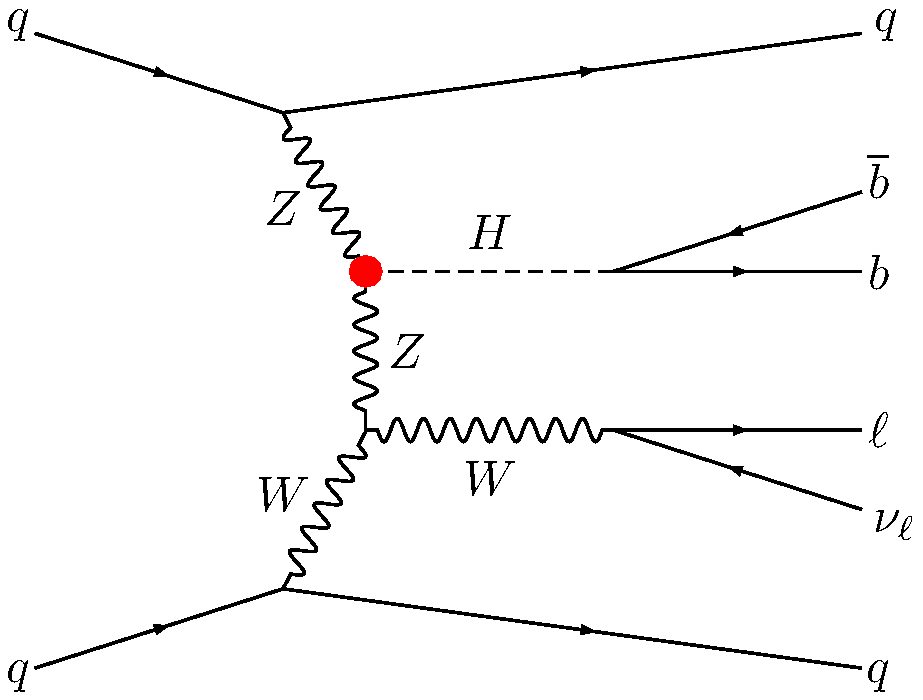
\includegraphics[width=0.3\textwidth]{fig/feynman/vbswh/vbswh_1.pdf}}\quad
    \subfloat{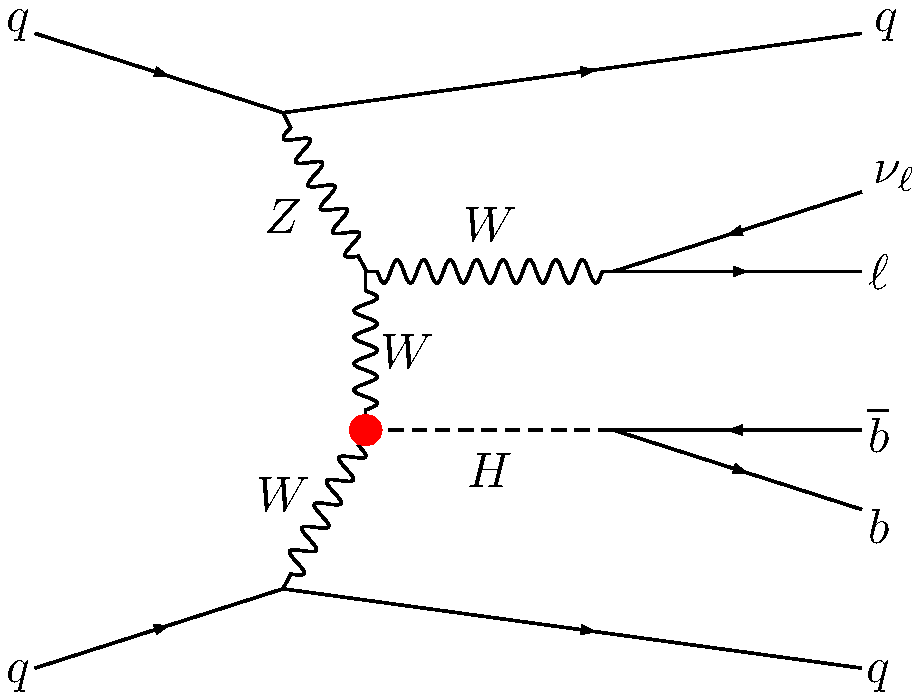
\includegraphics[width=0.3\textwidth]{fig/feynman/vbswh/vbswh_2.pdf}}\quad
    \subfloat{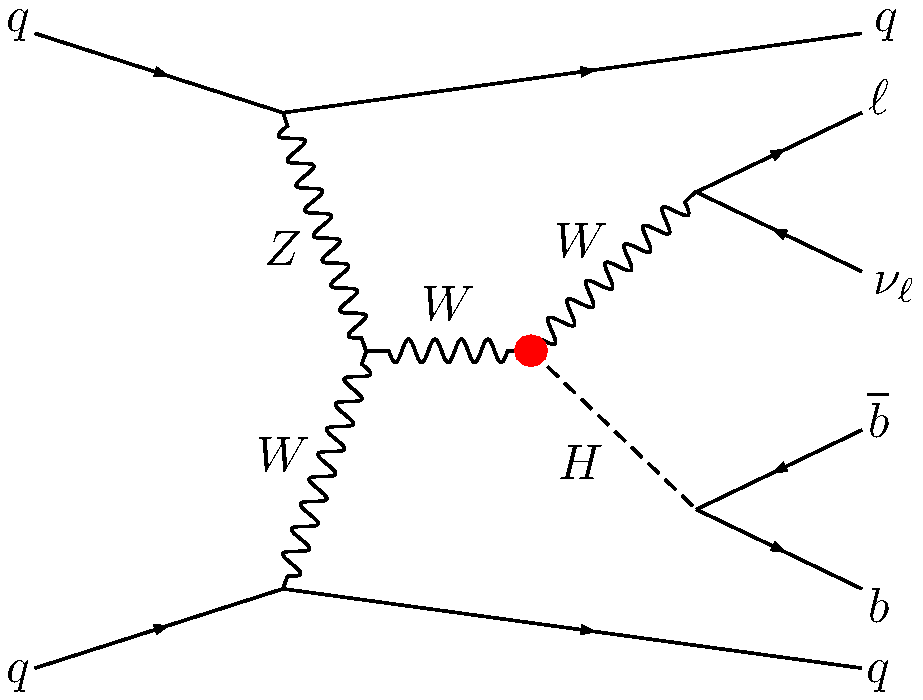
\includegraphics[width=0.3\textwidth]{fig/feynman/vbswh/vbswh_3.pdf}}
    \caption[Leading-order Feynman diagrams for VBS \WH production]{
        Leading-order Feynman diagrams for VBS production of a W and Higgs boson, where the W decays leptonically and the Higgs decays to b quarks. 
        The Higgs coupling to W bosons \kW and Z bosons \kZ is denoted by a red circle (\textcolor{red}{\ding{108}}). 
    }
    \label{fig:vbswh_feynman}
\end{figure}

\subsection{Signal characteristics}
A specific final state is intentionally selected for its uniqueness---making the signal easier to find amidst the haystack. 
First, leptons are preferred in the final state over jets, due to the sheer size of the ``QCD'' background, the most populous physics process produced at the LHC. 
Then, $\PW\to\ell\nu$ is preferred over $\PZ\to\ell\ell$, since there are fewer backgrounds with only one lepton in the final state. 
Finally, $\PH\to\PQb\PAQb$ has the largest branching ratio, and it can be identified using the latest advances in artificial intelligence. 

While there are a few, quite large background processes can produce the target final state, the Monte Carlo (MC) simulation of the signal reveals additional boons. 
The final state particles receive a significant boost for negative \lambdaWZ scenarios (Fig.~\ref{fig:vbswh_lhe}). 
In our preferred final state, this will give a lepton with large \pt, some additional \MET from the neutrino, and two overlapping b-jets reconstructed as a single merged jet. 
This can be quantified in a single variable by simply summing the \pt of each final-state particle other than the VBS jets:
\begin{equation}\label{eq:vbswh_st}
    \ST = \pt(\PW\to\ell\nu)+\pt(\Htobb) = \pt(\ell)+\ptmiss+\pt(\text{AK8 jet})
\end{equation}
The cross-section of the signal process increases almost quadratically as \kW or \kZ deviate from the SM value (Fig.~\ref{fig:vbswh_xsecs}), so there are simply more signal events in BSM scenarios. 
Importantly, the cross-section and Lorentz boost are the same for $\kW=-1$, $\kZ=1$ and $\kW=1$, $\kZ=-1$. 
The analysis was optimized for the latter case. 

\begin{figure}[htb]
    \centering
    \subfloat{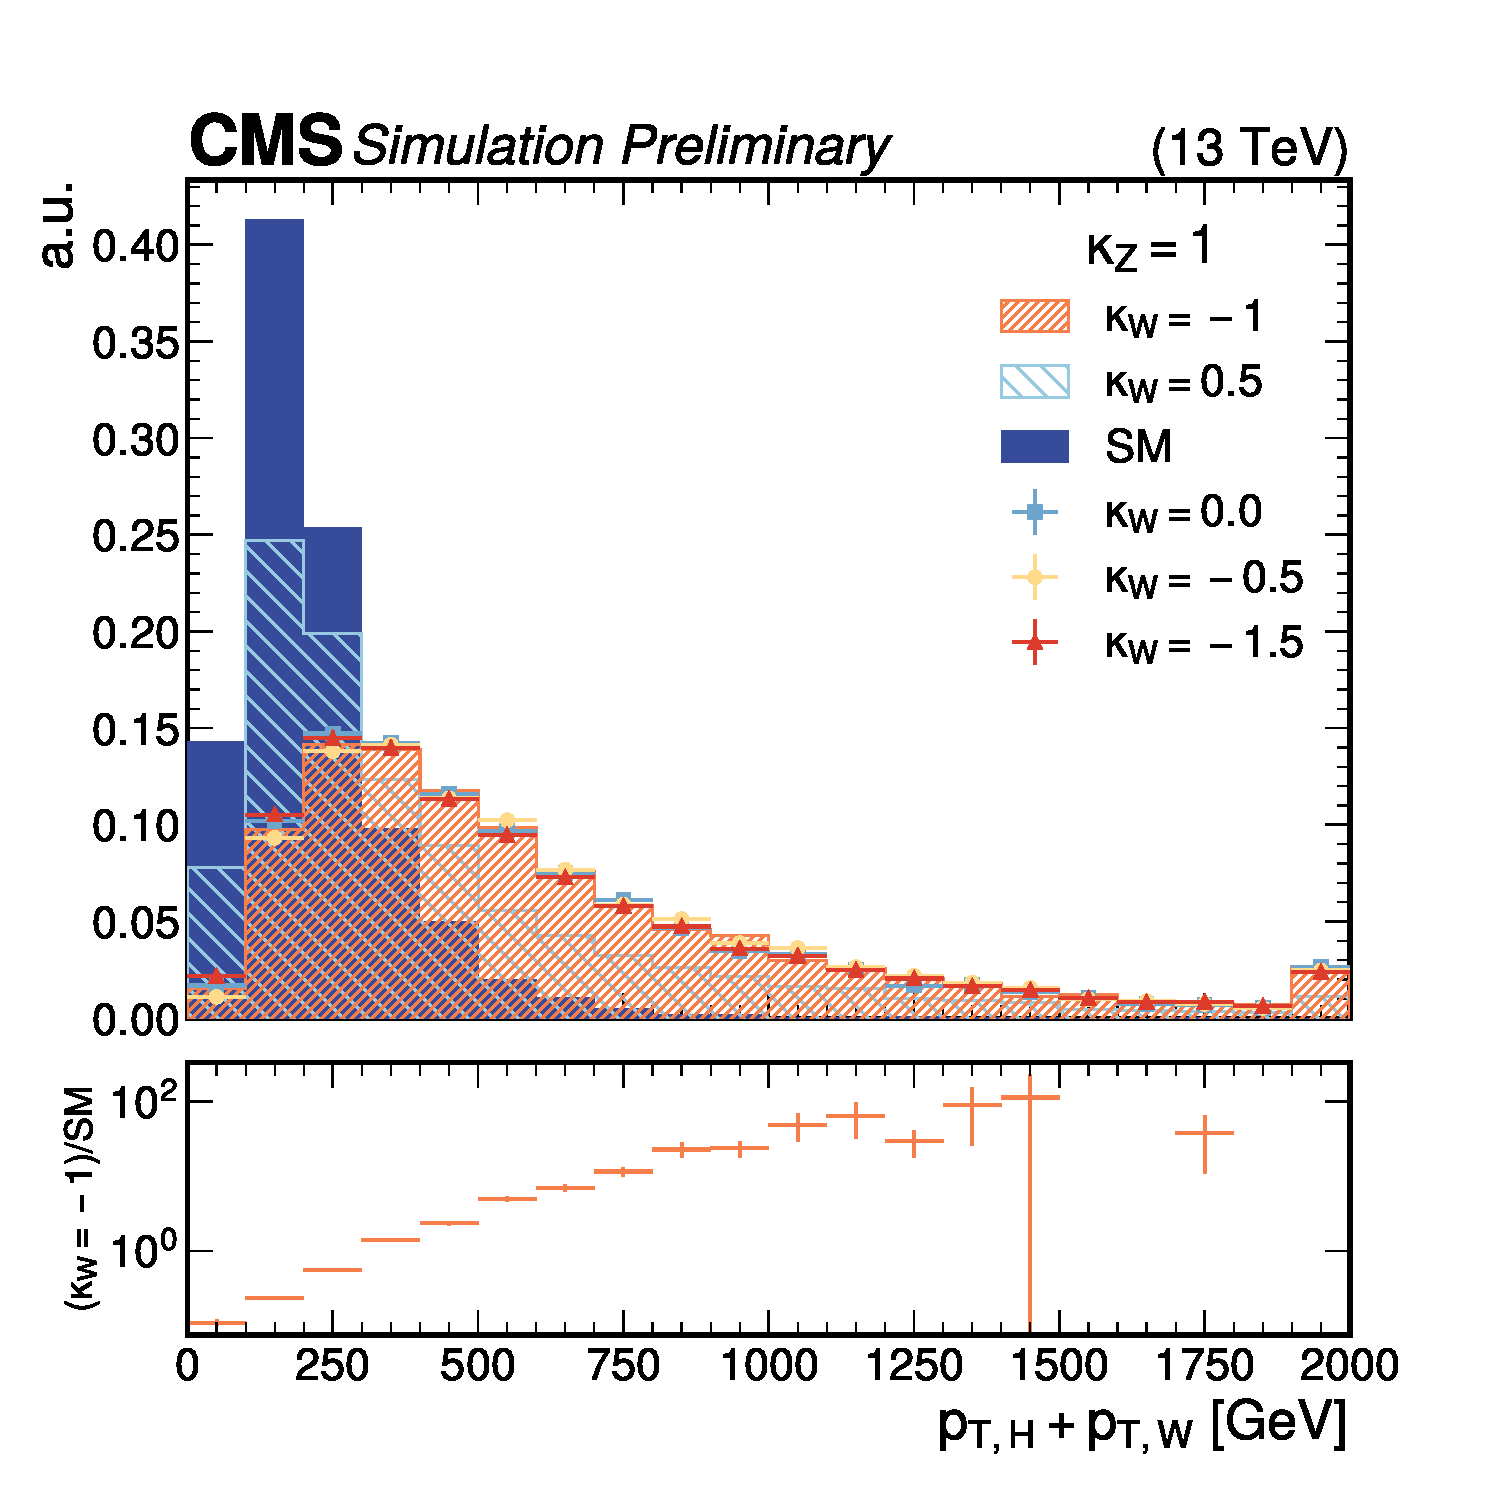
\includegraphics[width=0.45\textwidth]{fig/vbswh/lhe_ST_1p0kZ_kWpoints_norm.pdf}\label{fig:lheST_kWpoints}}
    \qquad
    \subfloat{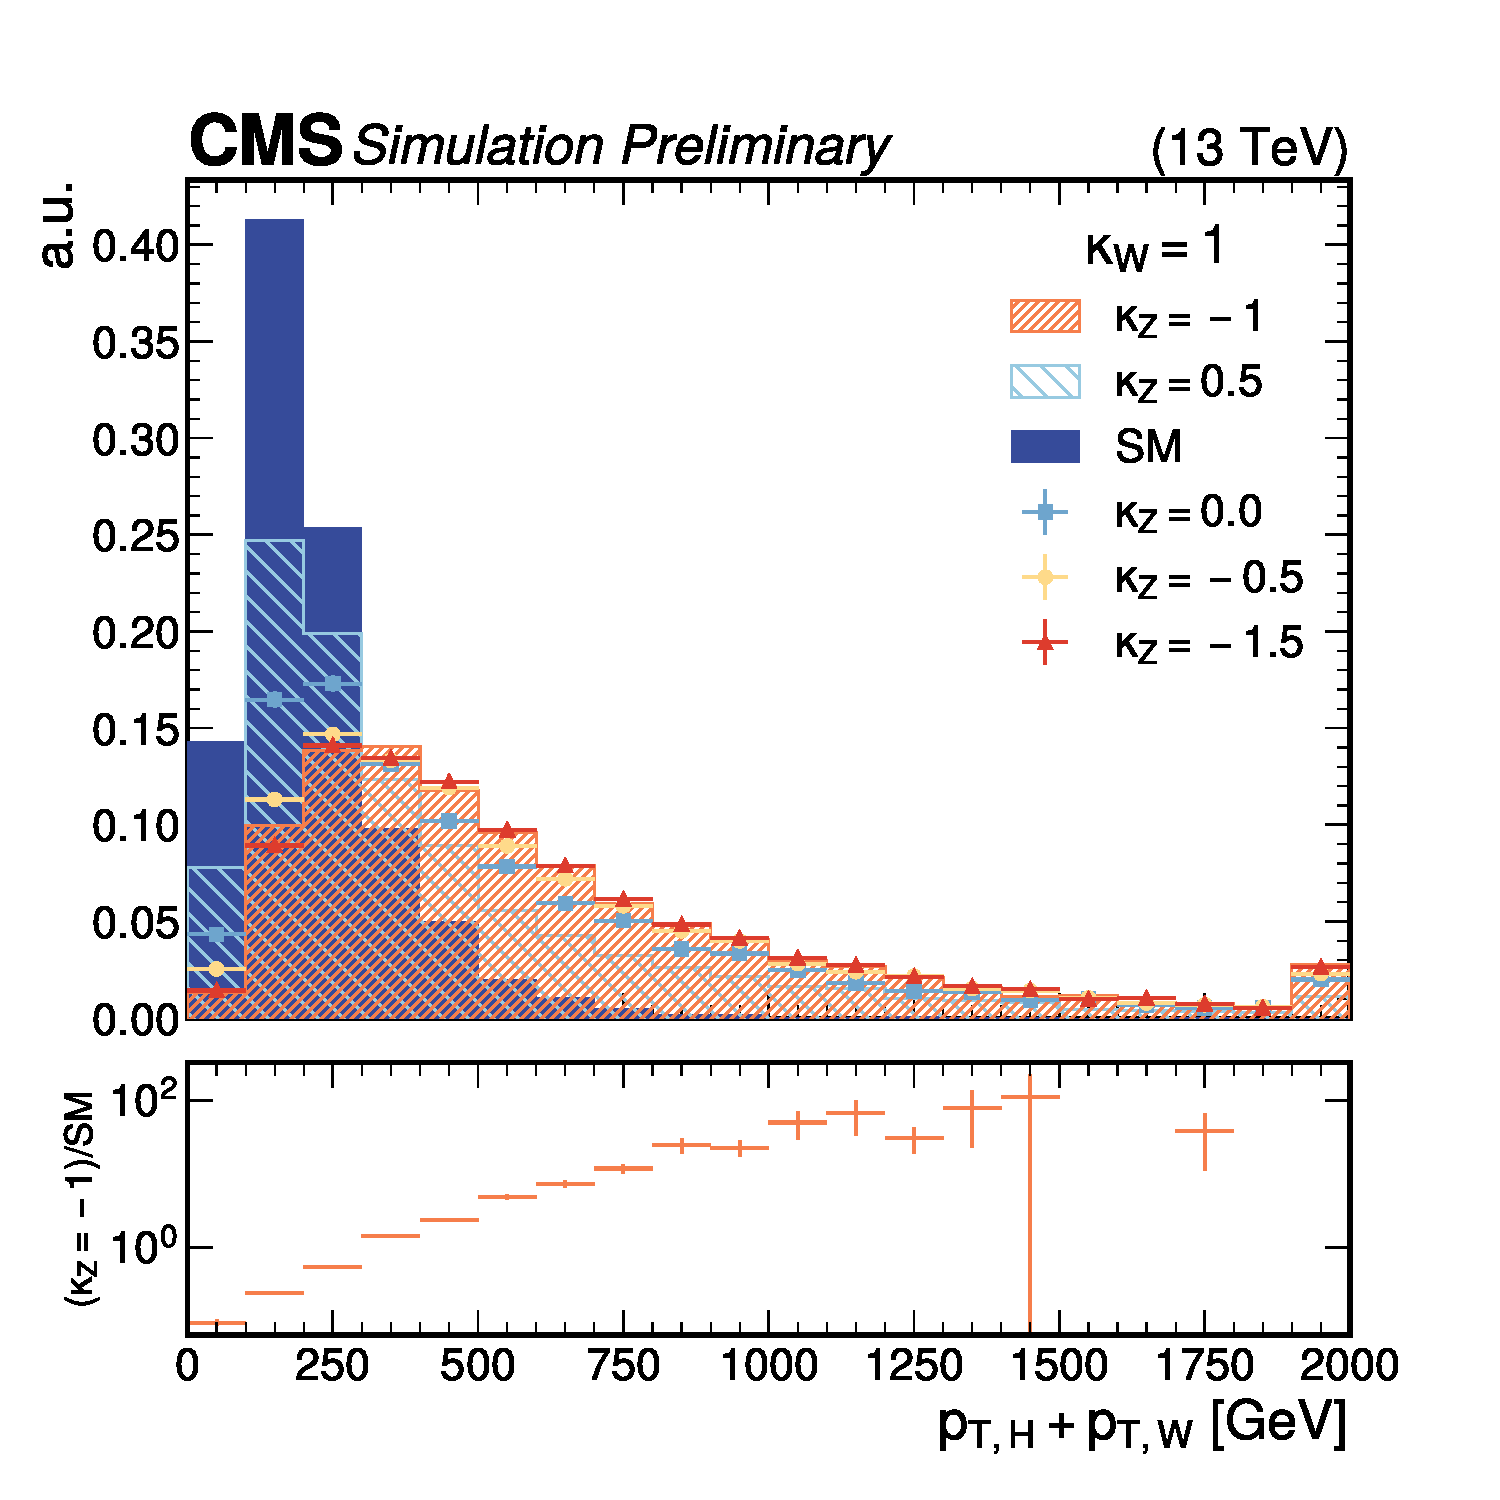
\includegraphics[width=0.45\textwidth]{fig/vbswh/lhe_ST_1p0kW_kZpoints_norm.pdf}\label{fig:lheST_kZpoints}}
    \caption[Generator-level \ST distribution]{
        Distribution of \ST plotted at the generator level for $\kZ = +1$ (left) and $\kW = +1$ (right), demonstrating the Lorentz boost in the final state due to modifications to \lambdaWZ. 
    }
    \label{fig:vbswh_lhe}
\end{figure}

\begin{figure}[htb]
    \centering
    \subfloat{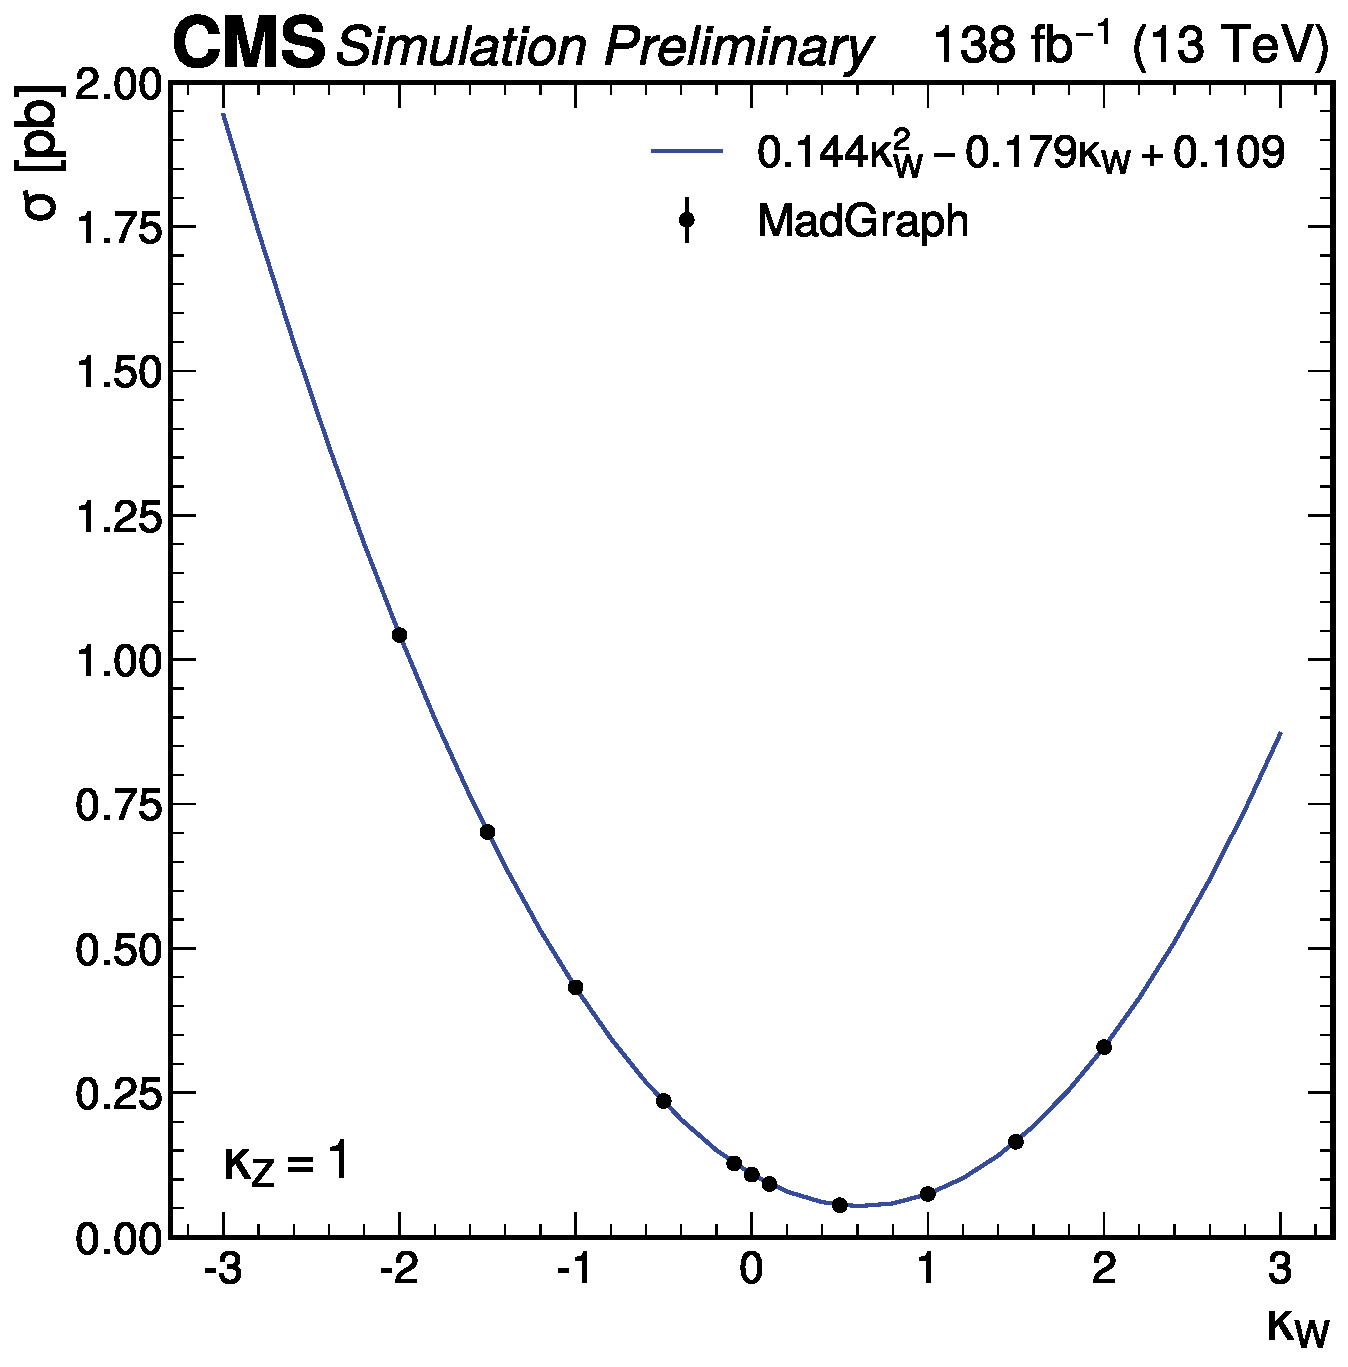
\includegraphics[width=0.45\textwidth]{fig/vbswh/kW_xsecs.pdf}}
    \qquad
    \subfloat{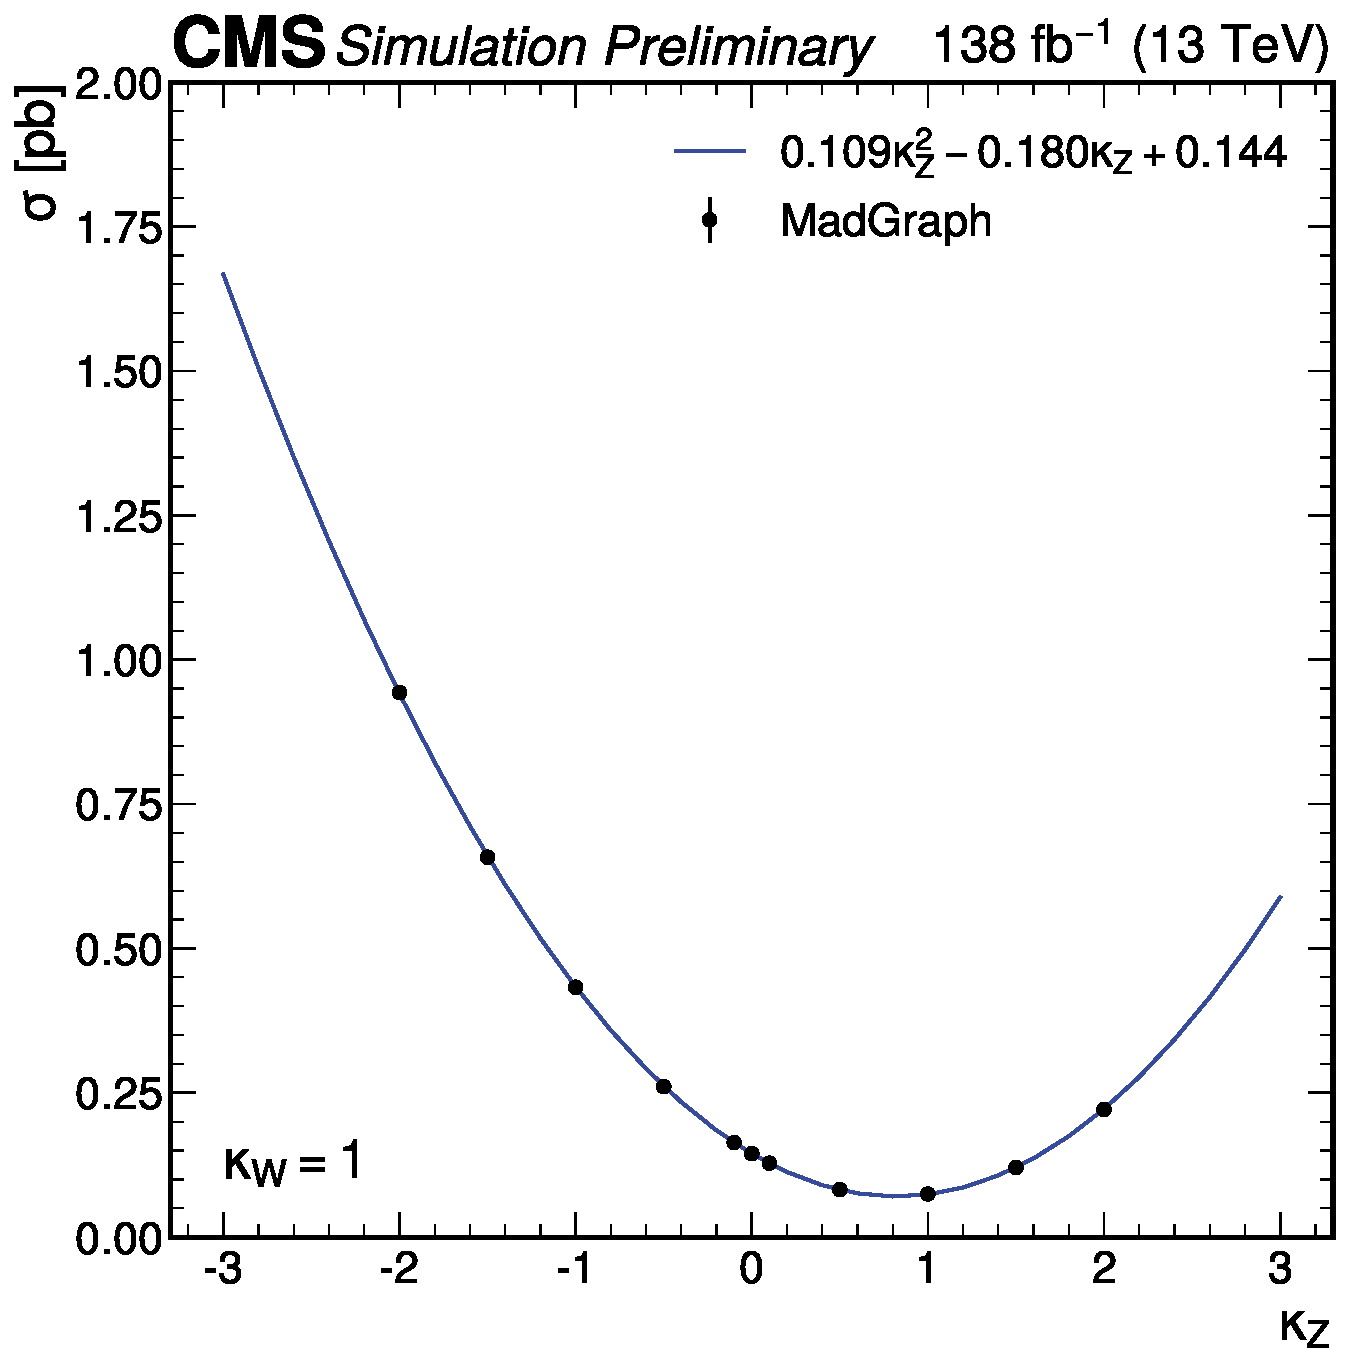
\includegraphics[width=0.45\textwidth]{fig/vbswh/kZ_xsecs.pdf}}
    \caption[The signal cross-section plotted as a function of enhancements to \kW]{
        The signal cross-section plotted as a function of enhancements to \kW, keeping $\kZ = +1$ (left) and to \kZ, keeping $\kW = +1$ (right). 
        The black points are taken from \MGvATNLO, and the blue curve is the best fit of a 2nd order polynomial to those points. 
    }
    \label{fig:vbswh_xsecs}
\end{figure}

The VBS jets also provide a distinct kinematic signature (Fig.~\ref{fig:vbswh_fireworks}), namely two nearly back-to-back jets---i.e. a large absolute difference in pseudorapidity \abs{\detajj}---with a large combined invariant mass \Mjj. 
In particular, the background processes fall off exponentially in \Mjj whereas the signal process is more flatly distributed. 
Combined with the fact that the signal has a distinctly larger average value of \abs{\detajj} than background, these VBS characteristics form a strong handle for distinguishing signal from background. 

\begin{figure}[htb]
    \centering
    \subfloat{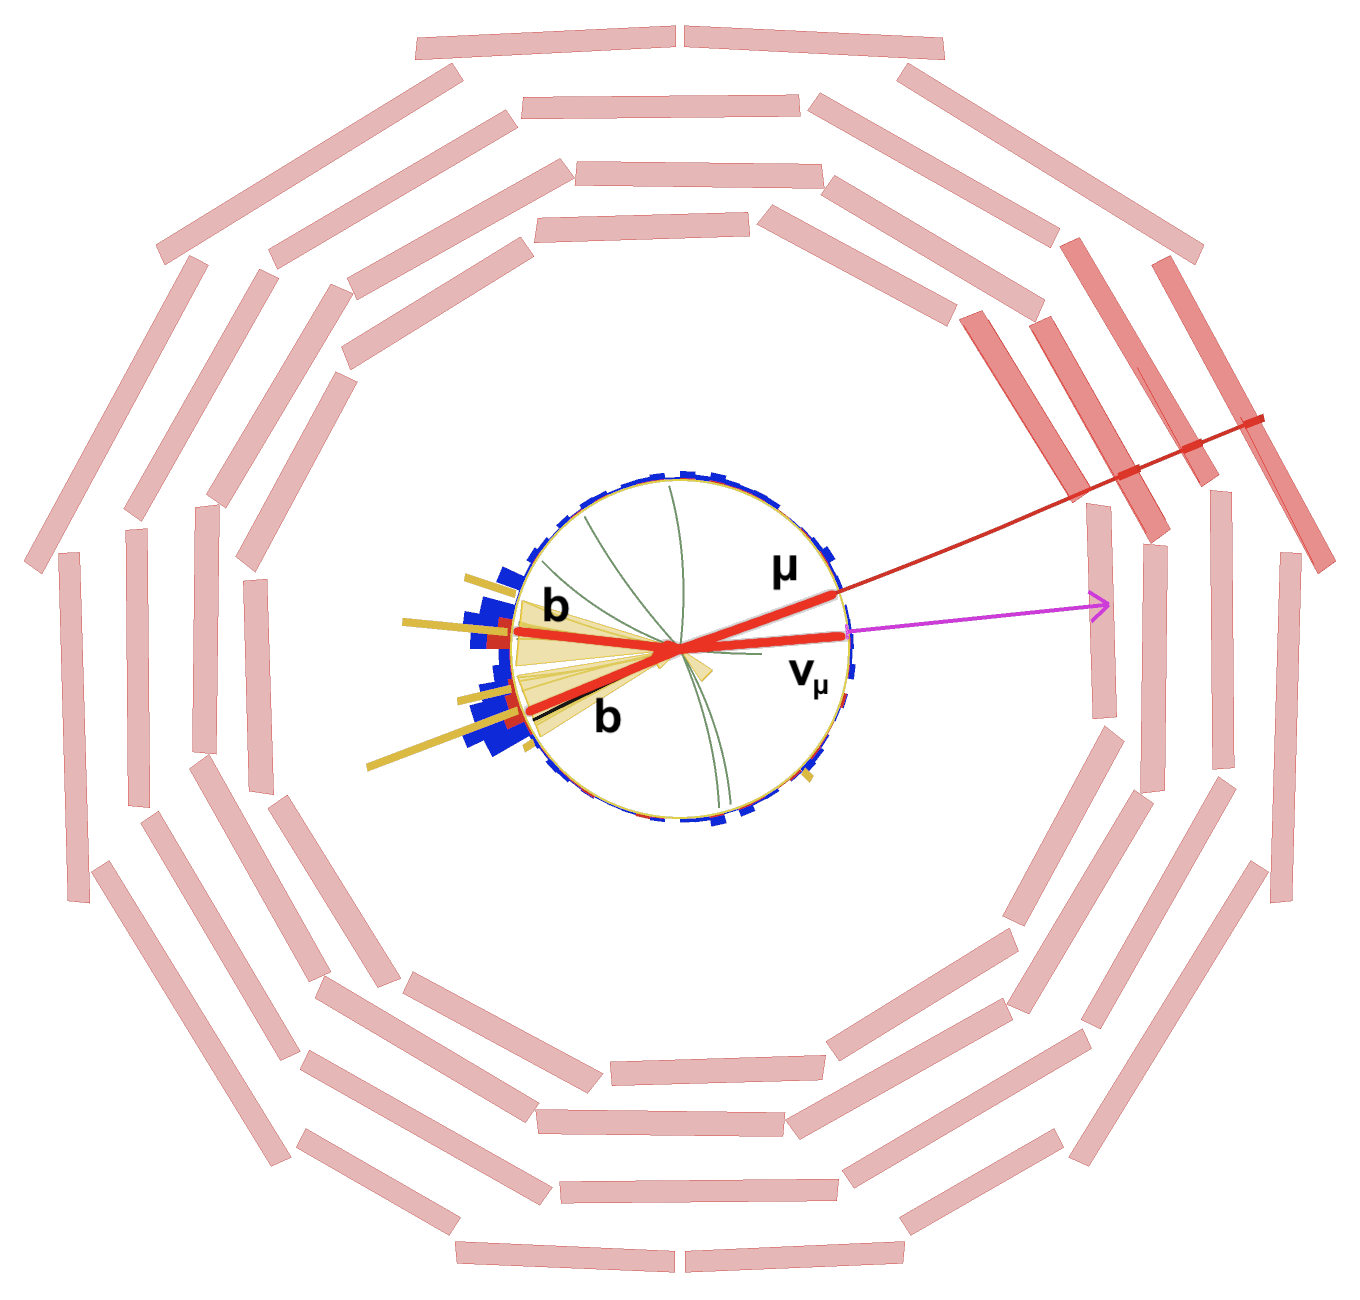
\includegraphics[width=0.45\textwidth]{fig/vbswh/fireworks/signal/vbswh_evt131104_rphi_gen_labeled.png}}
    \qquad
    \subfloat{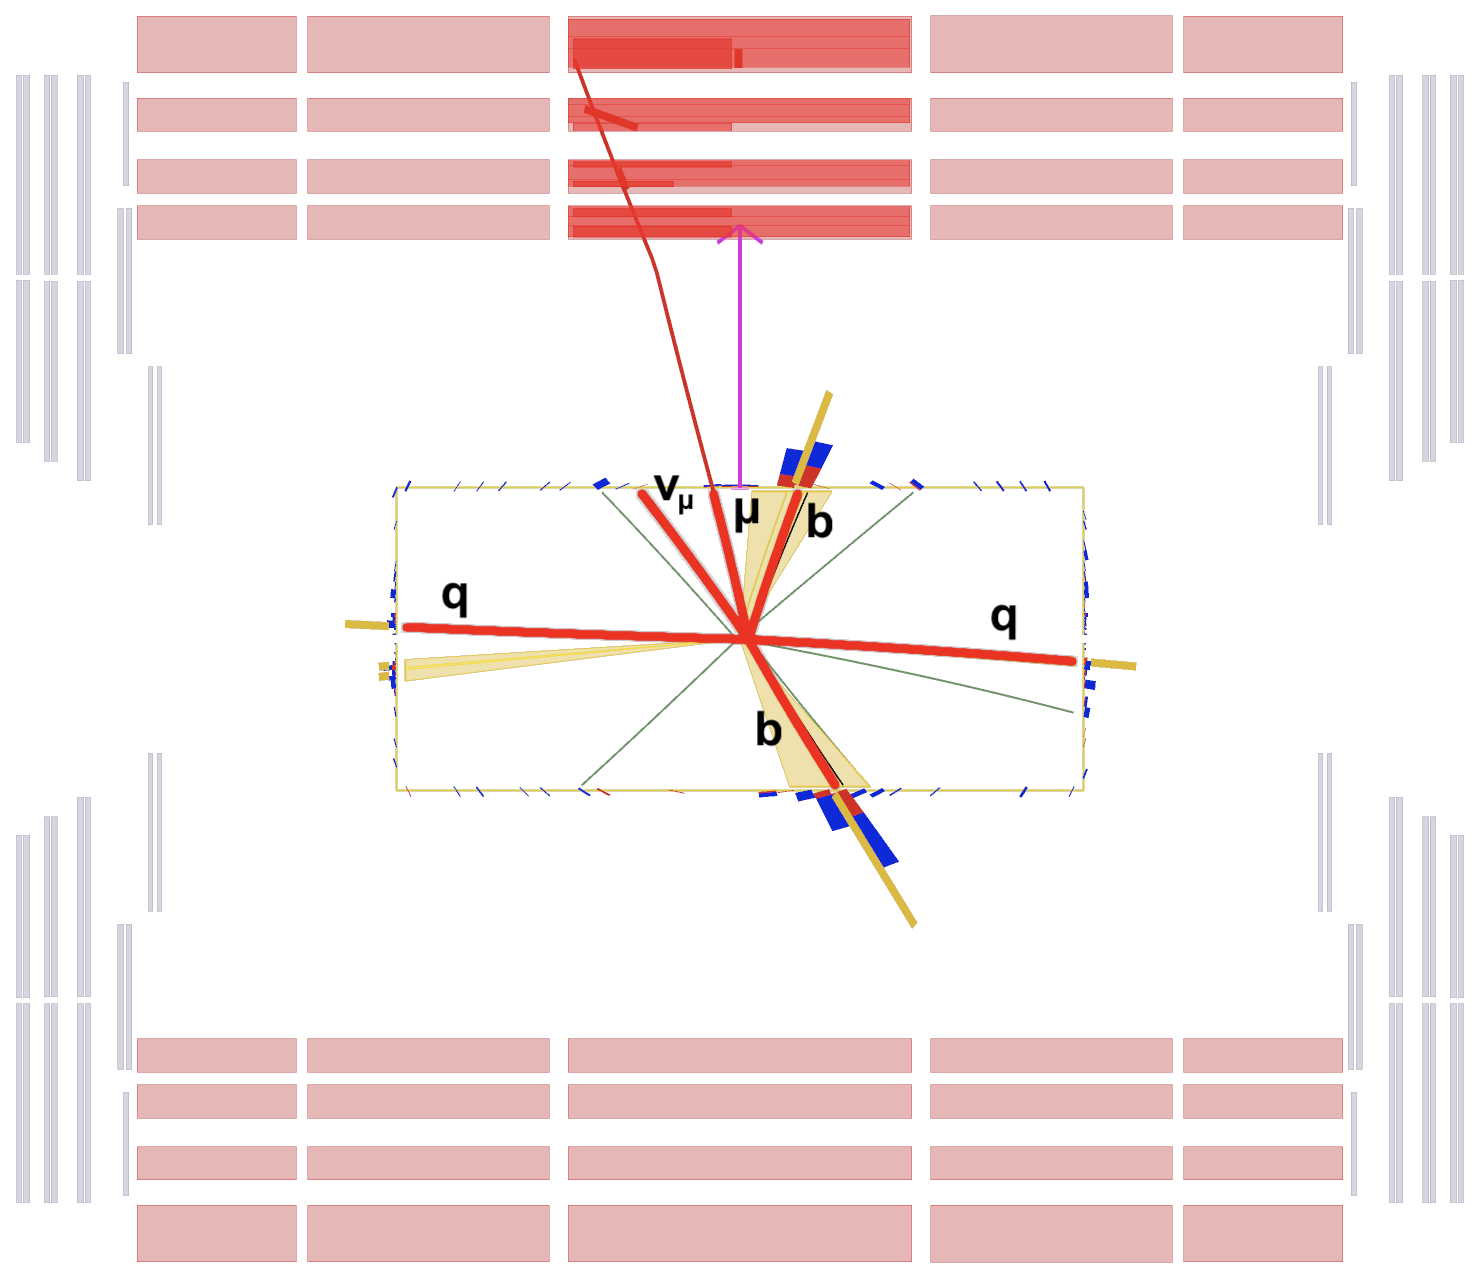
\includegraphics[width=0.45\textwidth]{fig/vbswh/fireworks/signal/vbswh_evt131104_rz_gen_labeled.png}}
    \caption[Event display for a simulated VBS \WH event]{
        Event display for a simulated VBS \WH event in the $r$-$\phi$ plane (left) and $r$-$z$ plane (right), with the final-state particles (thick red lines) labeled. 
        Two VBS jets can be seen very near to the beamline, going in either direction in $z$. 
    }
    \label{fig:vbswh_fireworks}
\end{figure}

\section{The backgrounds}
In general, background processes for this analysis need a fake\footnotemark{} $\Htobb$ merged jet, two fake\footnotemark[\value{footnote}] VBS jets, one lepton, and some \MET. 
\footnotetext{
    In principle, a background process could have a \textit{real} Higgs boson with large \pt decay to \bbbar or two \textit{real} VBS jets, however SM processes with these kinds of signatures are so rare that they do not represent a significant background for this analysis.
}
The leading background process for this analysis is \ttbar production, wherein a top and antitop quark are produced and both decay to a bottom quark and \PW boson. 
One of the \PW bosons can decay to a real lepton and neutrino, and the fake VBS jets and \Htobb merged jet can come from some combination of the \PQb quarks, quarks from one of the \PW bosons decaying hadronically, and possibly an extra gluon radiated by one of the incoming quarks (Fig.~\ref{fig:ttbar1l}). 
One of the incoming quarks can also radiate a \PW or \PZ boson (Fig.~\ref{fig:ttV1l}), which presents additional opportunities for trickery. 
The largest sub-leading background comes from \wjets (Fig.~\ref{fig:w_jets}), where a \PW boson is produced along with some number of quarks or gluons, and single-top production (Fig.~\ref{fig:single_t}), where only one top quark is produced. 
In \wjets, the W can give a real lepton and neutrino, while the additional jets cover the fake VBS and \Htobb signature. 
In single-top production, the top quark again decays to a \PW boson and b quark, so it can produce a signal-like final state much like \ttbar. 

\begin{figure}[htb]
    \centering
    \subfloat[$\ttbar + \text{jet}$]{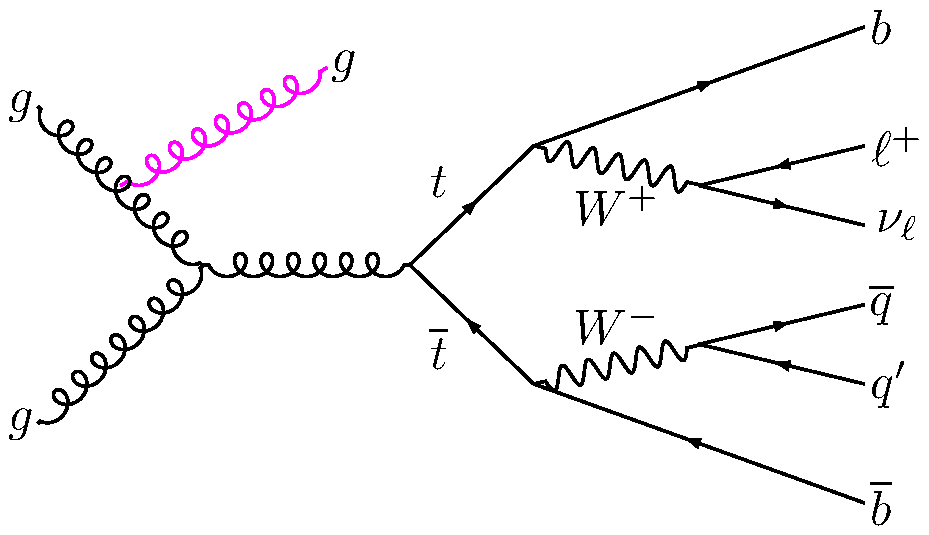
\includegraphics[width=0.4\textwidth]{fig/feynman/ttbar/ttbar_onelep_extraJet_ggF.pdf}\label{fig:ttbar1l}}
    \quad
    \subfloat[$\ttbar + \PV$]{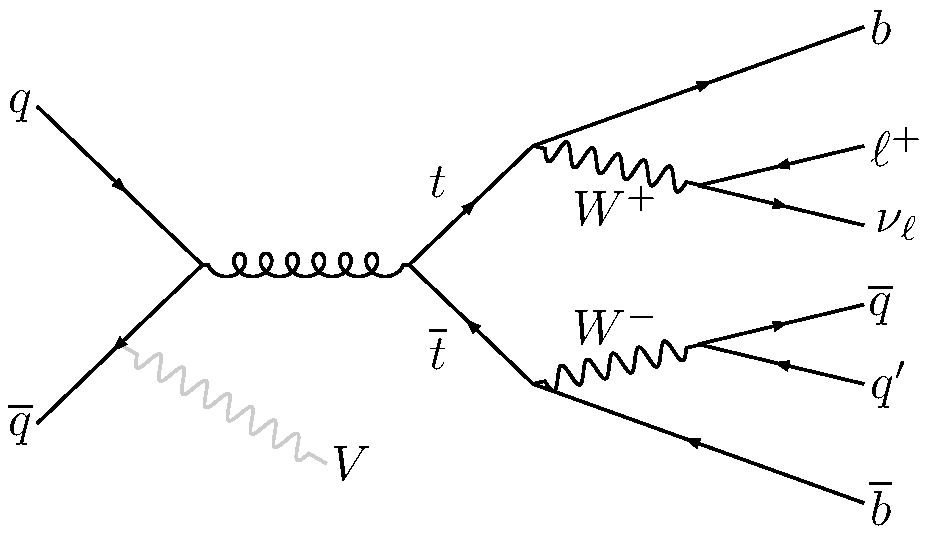
\includegraphics[width=0.4\textwidth]{fig/feynman/ttbar/ttV_onelep.pdf}\label{fig:ttV1l}}
    \\
    \subfloat[\wjets]{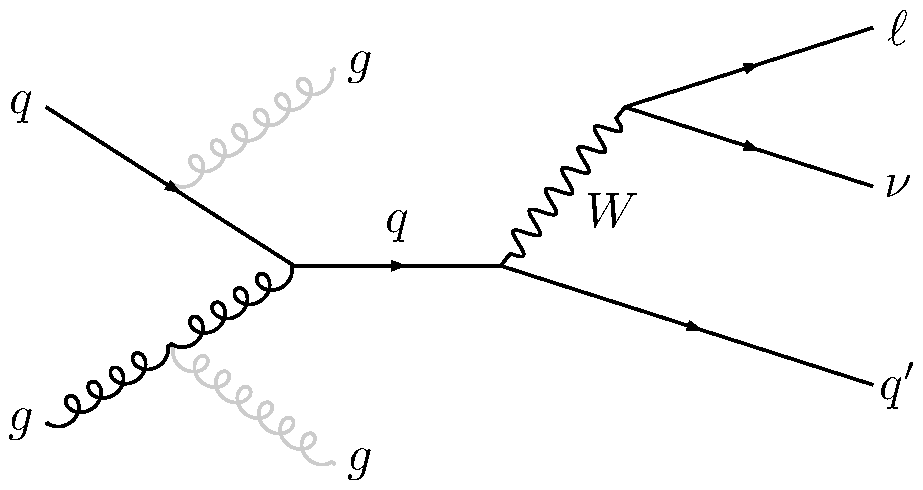
\includegraphics[width=0.4\textwidth]{fig/feynman/other/wjets.pdf}\label{fig:w_jets}}
    \quad
    \subfloat[Single top]{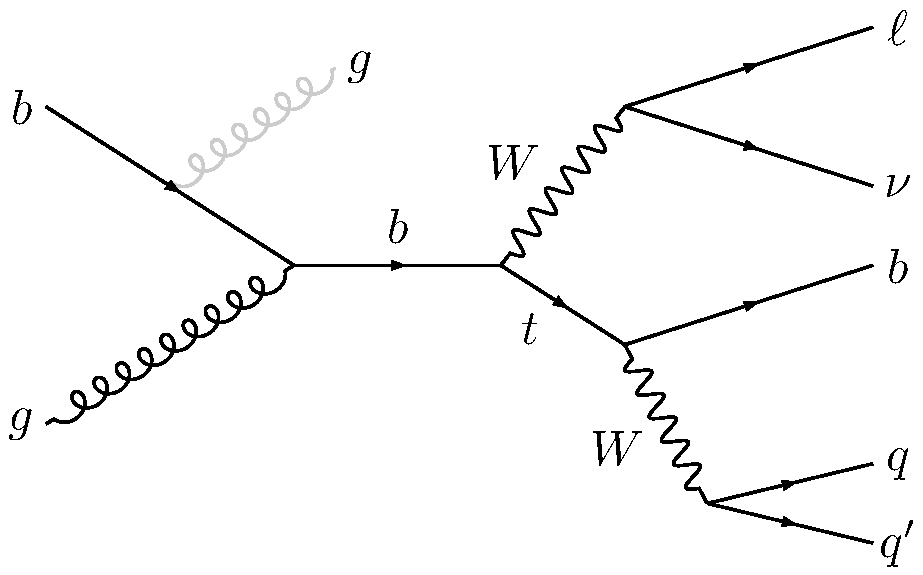
\includegraphics[width=0.4\textwidth]{fig/feynman/other/singletop_tW.pdf}\label{fig:single_t}}
    \caption[Feynman diagrams the leading (\ttbar) and subleading (\wjets and single top quark) backgrounds]{
        Feynman diagrams for the leading and subleading backgrounds in this analysis.
        From top to bottom: 
        \ttbar production in the single-lepton final state with (a) an extra jet from a gluon or (b) an extra vector boson ($\PV = \PW$ or \PZ) radiated from one of the incoming partons;  
        \wjets production in the single-lepton final state (c); and the production of a single top quark and \PW boson (d). 
    }
    \label{fig:vbswh_bkg}
\end{figure}

\section{Event selection}
\subsection{Triggers and preselection}
The single lepton in our signal final state gives a clean signature on which to trigger, so the aptly named ``single lepton'' triggers are applied and the ``single lepton'' datasets are used. 
These triggers are nearly 100\% efficient for signal events because the lepton in the BSM final state is expected to have high \pt. 
A number of additional event-level filters are applied to remove detector noise and unphysical events~\cite{JMEPaper}. 

Then, a loose selection, referred to as the ``Preselection,'' is applied to select the final state of interest. 
First, a loose selection is made on the combined VBS jet invariant mass: $\Mjj > 500\GeV$.
Next, the \ParticleNet \Xtobb score of the \Htobb fat jet candidate is required to be greater than 0.3.
The event is also required to have no AK4 jets passing the Medium \DeepJet working point.
The event must furthermore have one and only one lepton with $\pt > 40\GeV$ that passes the Tight lepton ID. 
If there are any additional leptons that pass the Veto lepton ID, the event is vetoed--these leptons are not required to pass the \pt threshold. 
Finally, the event must have $\ST > 800\GeV$ (where \ST is defined in Eq.~\ref{eq:vbswh_st}).

\subsection{Signal region}
The signal region for this analysis is defined on top of the Preselection with similar, but tighter selections. 
First, the \ST threshold is increased to $\ST > 900\GeV$. 
Then, the selections on the VBS jet variables are tightened to $\Mjj > 600 \GeV$ and $|\detajj| > 4$. 
Finally, the selections on the \Htobb fat jet candidate are made much more stringent, where the \ParticleNet \Xtobb score is required to be greater than 0.9 and \MSD is required to be less than 150\GeV. 

The background in this region is estimated using a data-driven technique, described in the next section, that the signal region was specifically designed to enable. 
Looser cuts are preferred in particular, as it was found that the variables used for the background estimation become correlated in a more restricted phase space. 
Therefore, the signal region selections are not optimized for maximal purity, though such a region can be formed. 

\begin{figure}[htb]
    \centering
    \subfloat{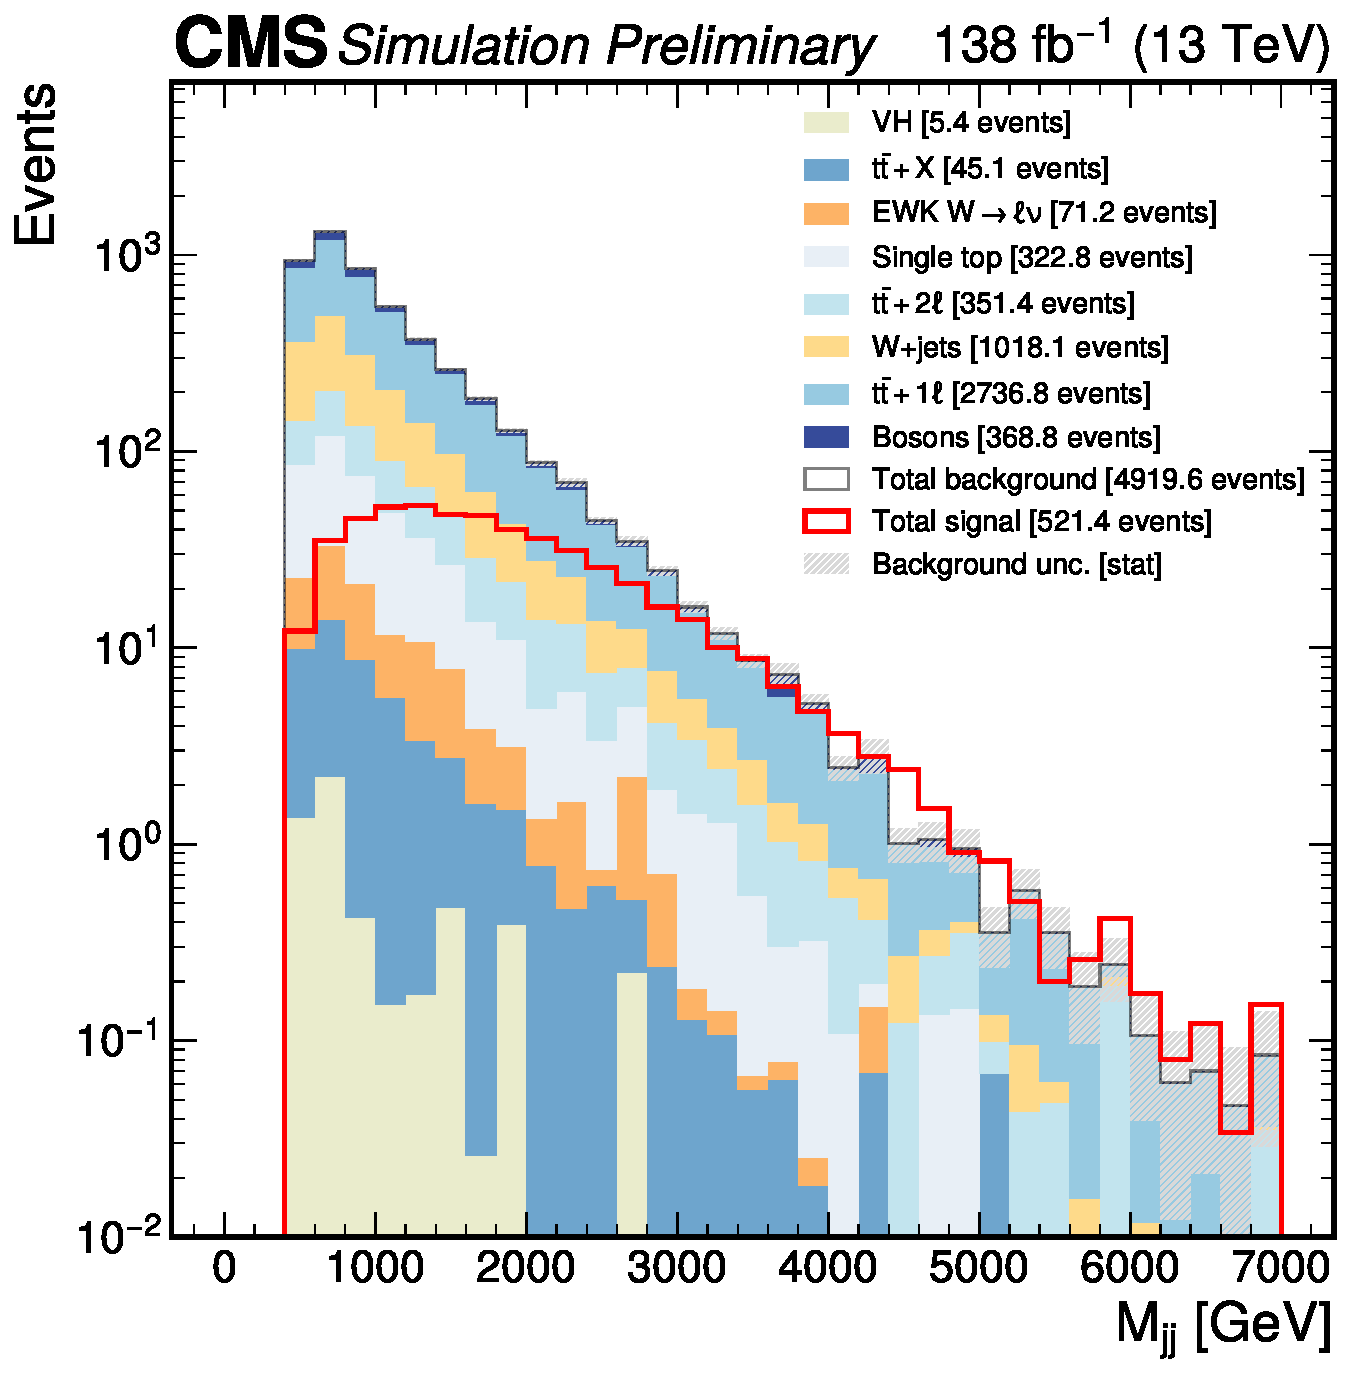
\includegraphics[width=0.45\textwidth]{fig/vbswh/M_jj_sig_vs_bkg_stacked_logy_presel_noDetaJJ.pdf}}
    \qquad
    \subfloat{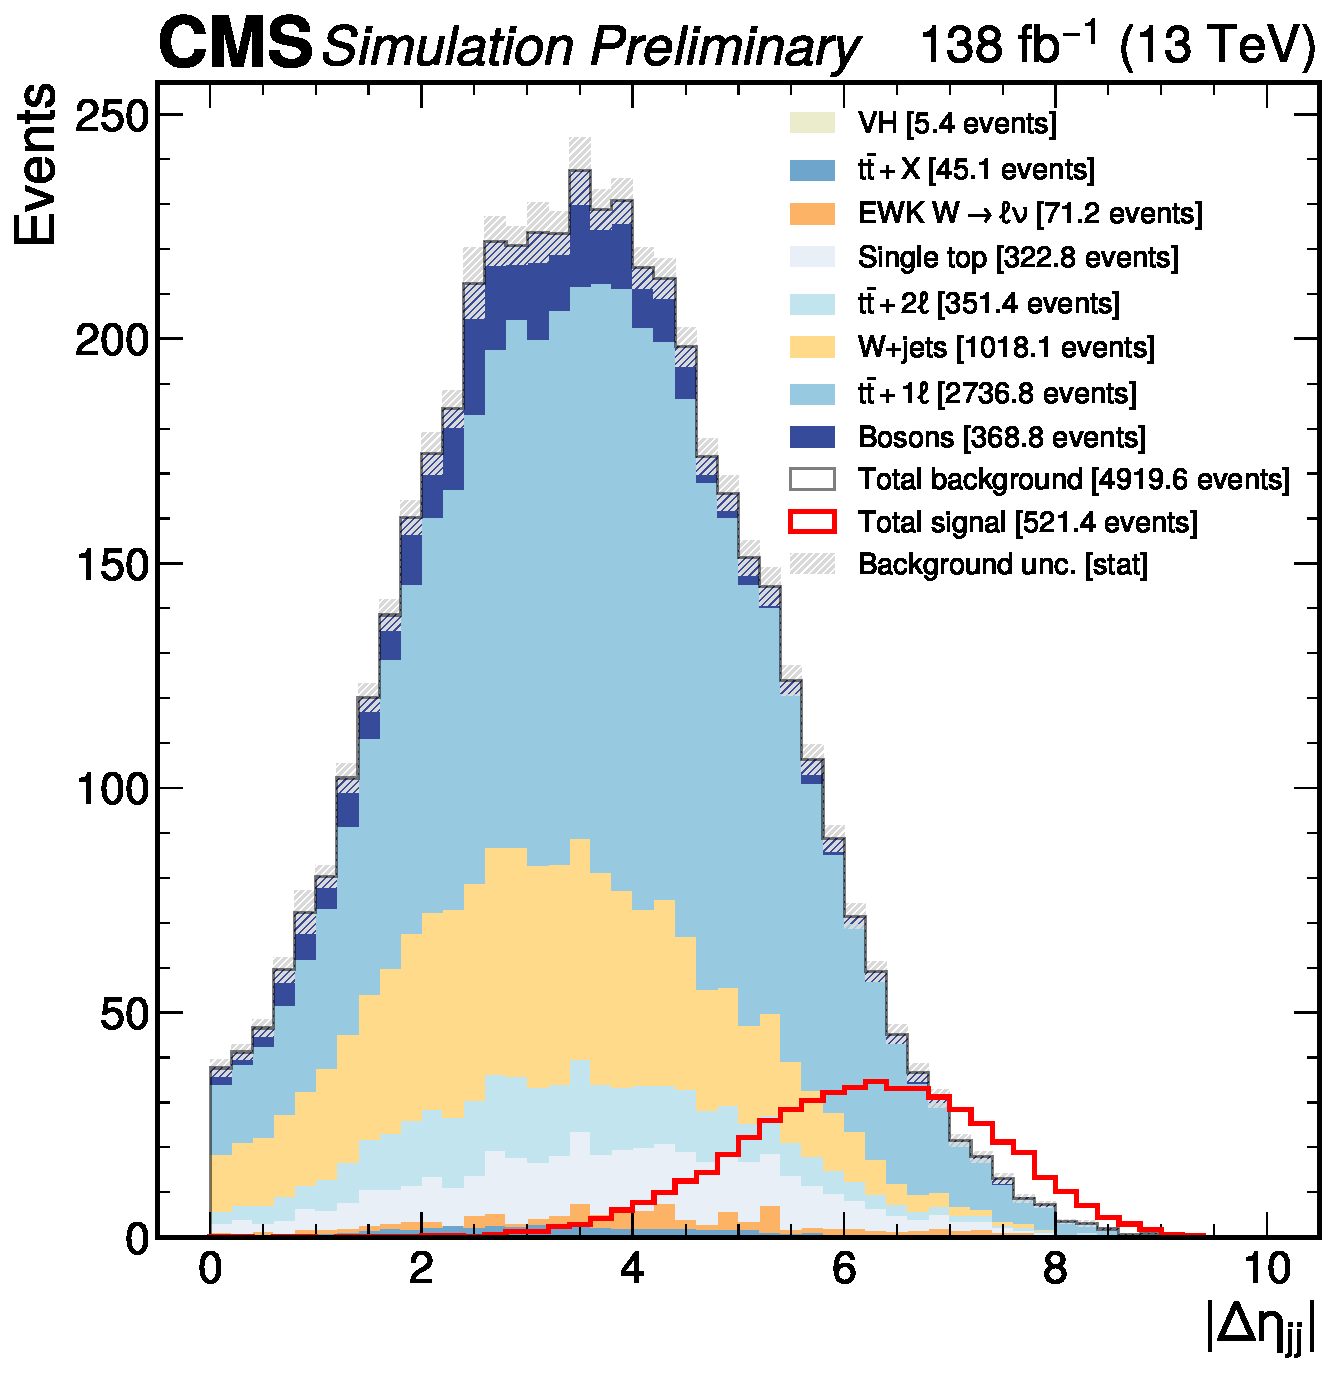
\includegraphics[width=0.45\textwidth]{fig/vbswh/deta_jj_sig_vs_bkg_stacked_presel_noDetaJJ.pdf}}
    \caption[The \Mjj and \detajj distributions for the VBS jets]{
        The VBS jet combined invariant mass \Mjj (left) and absolute difference in pseudorapidity $\abs{\detajj}$ (right) plotted after applying the Preselection.
    }
    \label{fig:vbswh_presel_vbs}
\end{figure}

\begin{figure}[htb]
    \centering
    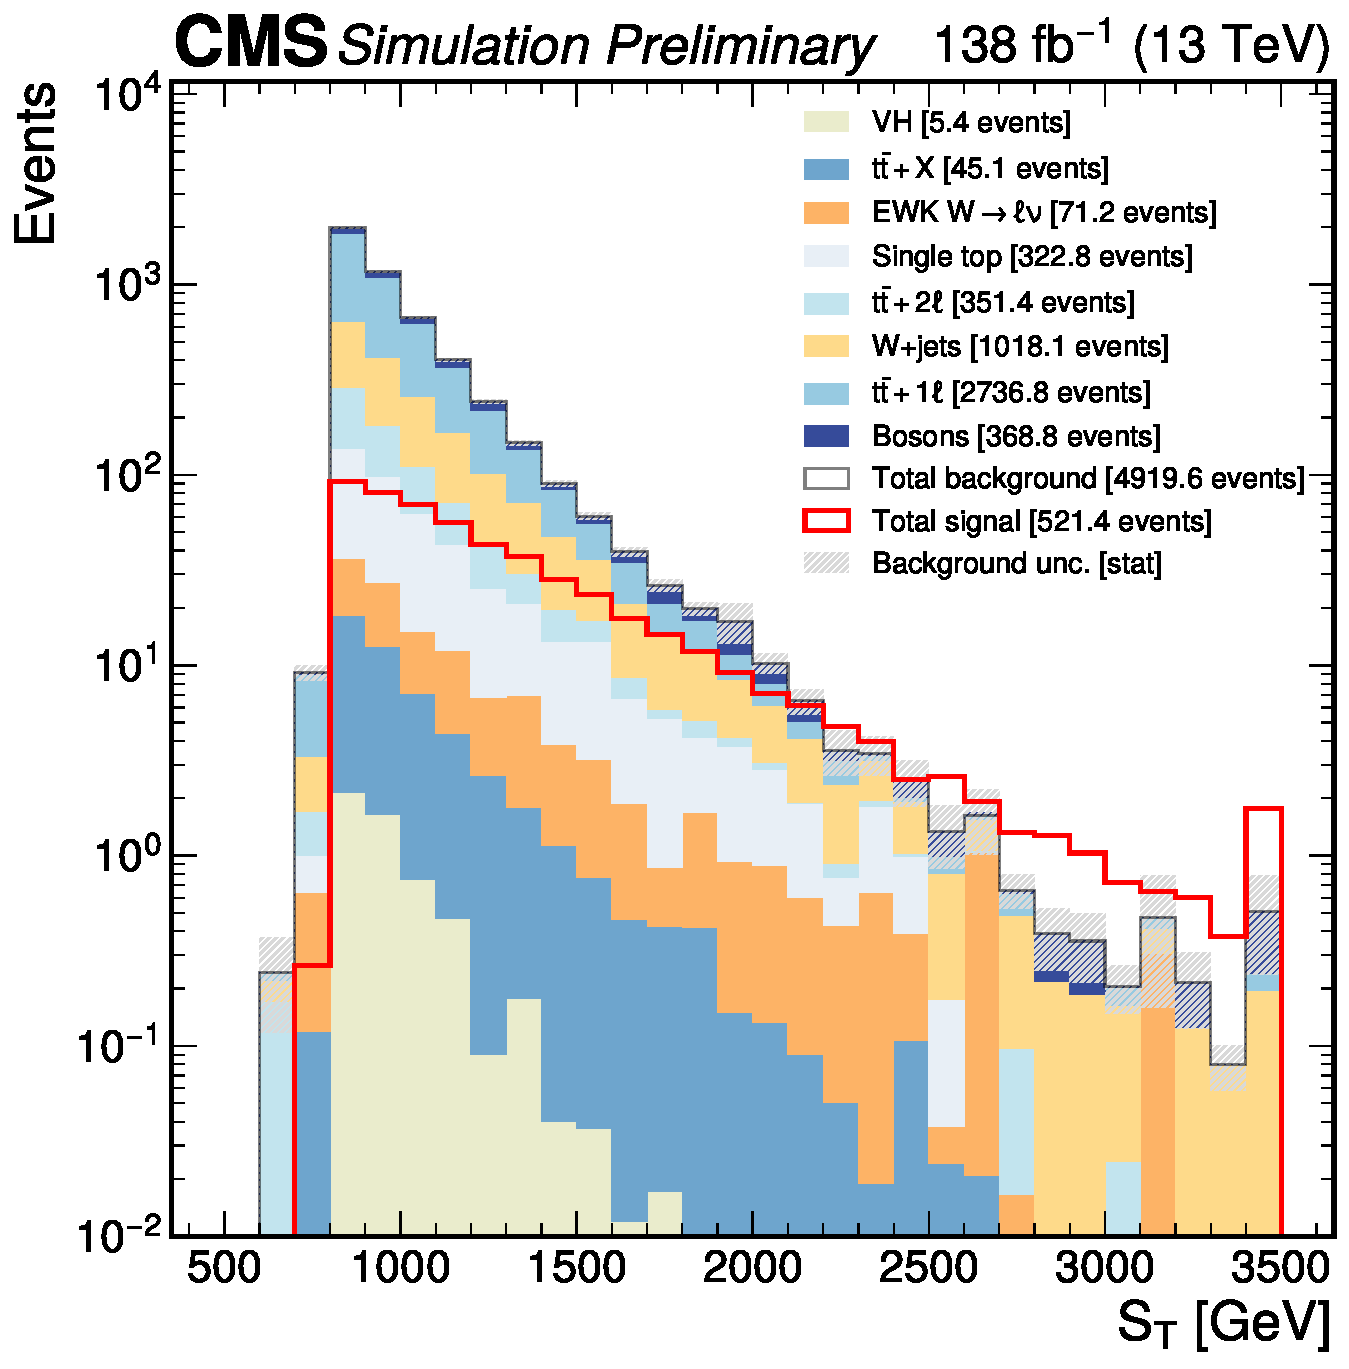
\includegraphics[width=0.45\textwidth]{fig/vbswh/ST_sig_vs_bkg_stacked_logy_presel_noDetaJJ.pdf}
    \caption[The \ST distribution]{
        The variable $\ST = \pt(\PH) + \pt(\ell) + \ptmiss$ plotted after applying the Preselection.
    }
    \label{fig:vbswh_presel_st}
\end{figure}

\begin{figure}[htb]
    \centering
    \subfloat{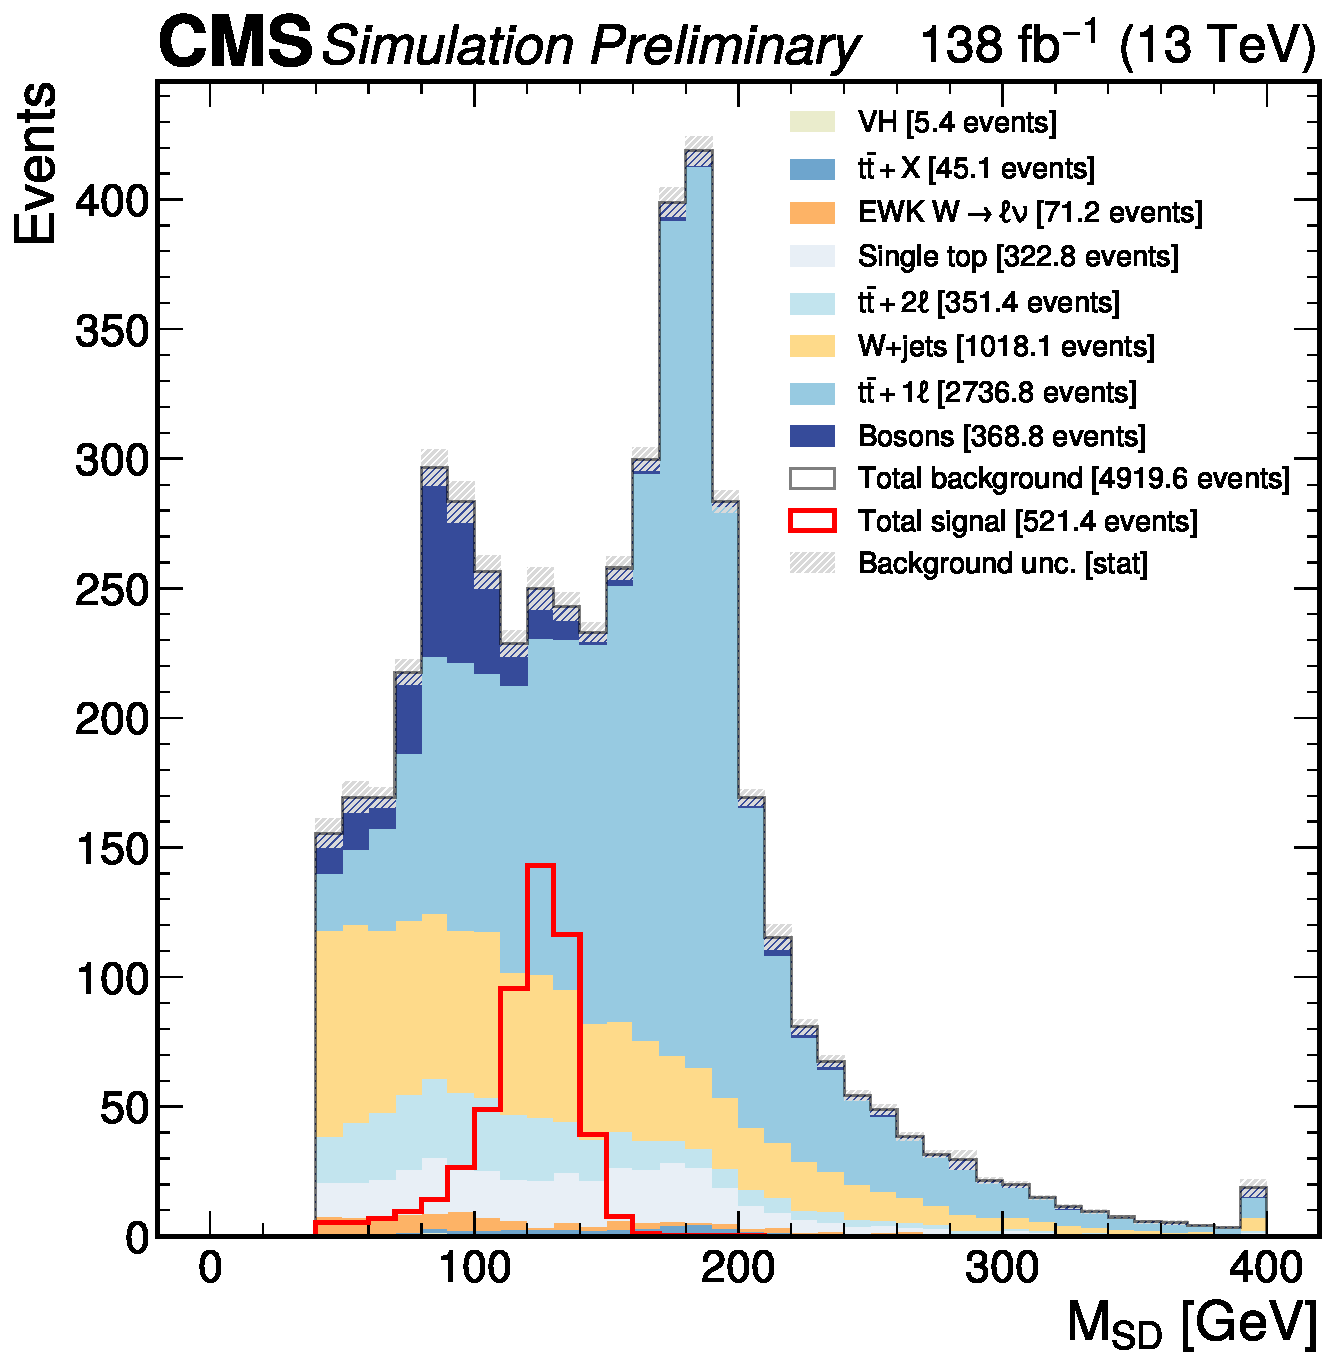
\includegraphics[width=0.45\textwidth]{fig/vbswh/hbbjet_msoftdrop_sig_vs_bkg_stacked_presel_noDetaJJ.pdf}}
    \qquad
    \subfloat{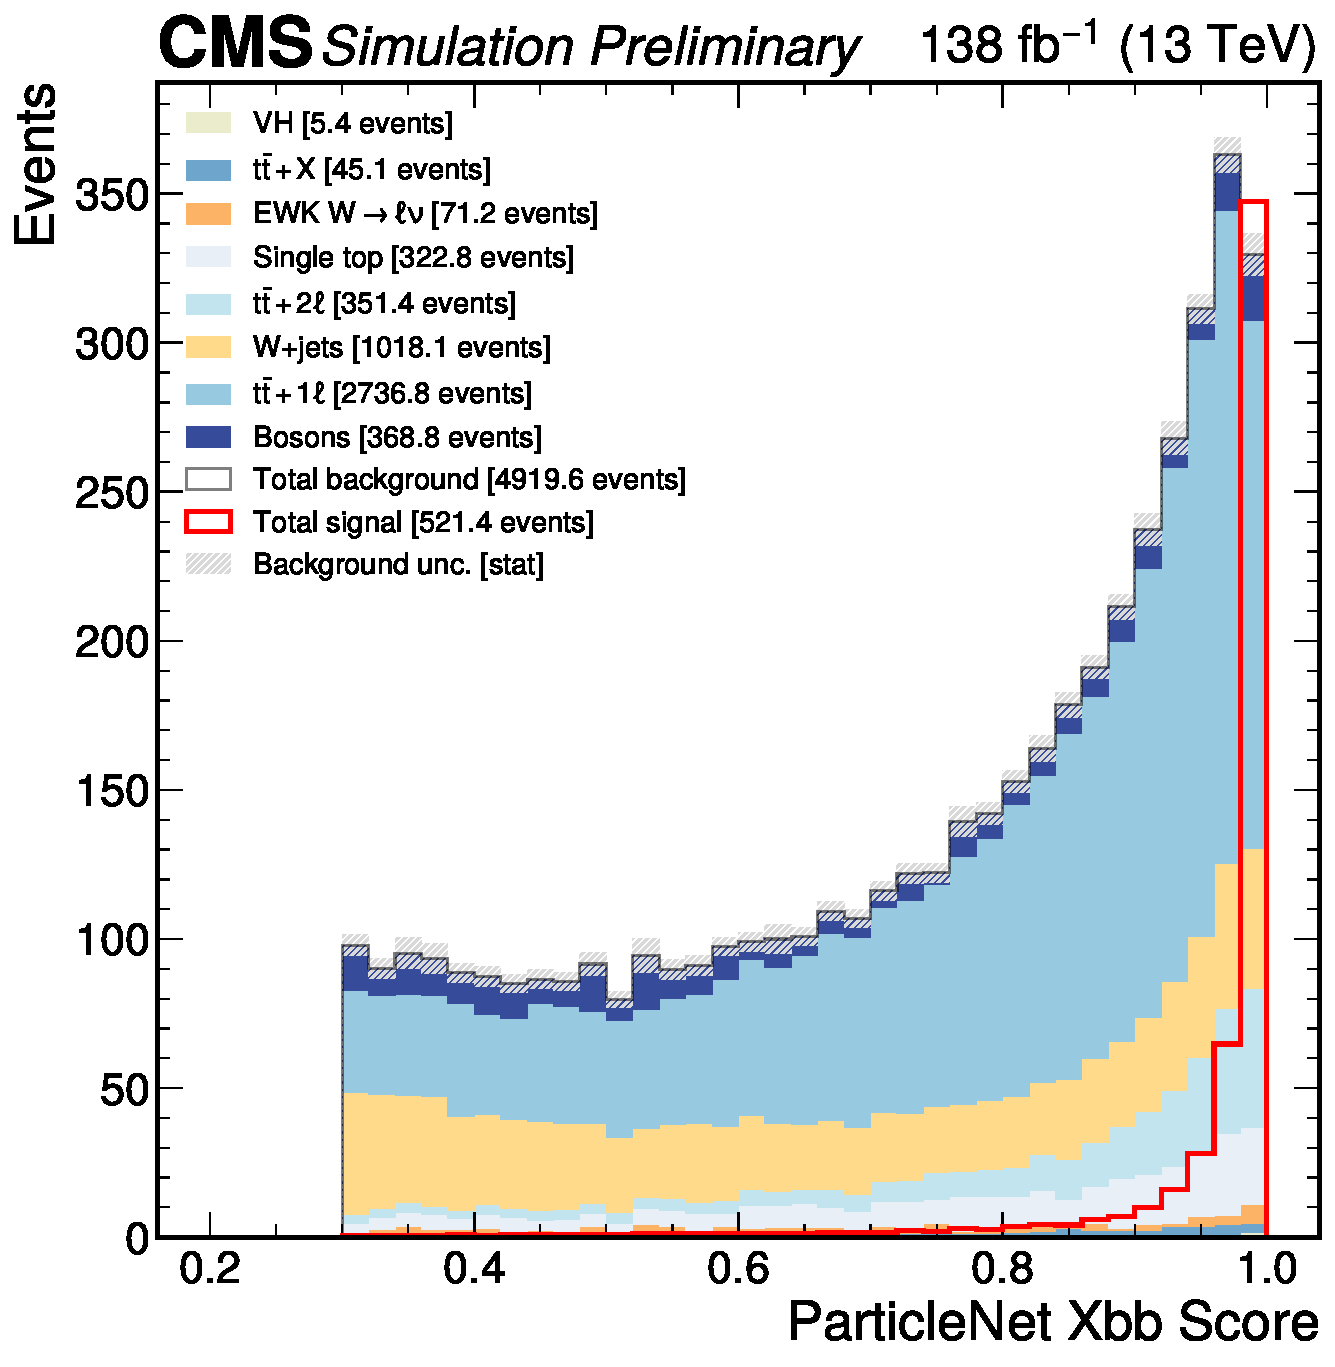
\includegraphics[width=0.45\textwidth]{fig/vbswh/hbbjet_score_sig_vs_bkg_stacked_presel_noDetaJJ.pdf}}
    \caption[The \Htobb fat jet candidate soft drop mass and \ParticleNet \Xtobb score distributions]{
        The \Htobb fat jet candidate soft drop mass (left) and \ParticleNet \Xtobb score (right) plotted after applying the Preselection.
    }
    \label{fig:vbswh_presel_hbb}
\end{figure}

\section{Background estimation}
The background in the signal region is estimated using the ``ABCD'' method, where region A is the signal region, and regions B, C, and D have the \detajj requirement, the \MSD requirement, and both inverted, respectively (Fig.~\ref{fig:vbswh_abcd_cartoon}). 
First, let the background yield in regions A, B, C, and D in Monte Carlo be defined as \AMC, \BMC, \CMC, and \DMC.
Likewise, let the same yields in data be defined as  \Adata, \Bdata, \Cdata, and \Ddata.
Under these definitions, the estimated background yield in region A, referred to as \AdataPred, can be computed with data as follows:
\begin{equation}\label{eq:vbswh_abcd}
    \AdataPred = \Bdata\times\frac{\Cdata}{\Ddata}
\end{equation}
\noindent where the same can be done in MC, yielding \AMCPred. 
First, it can be seen in Fig.~\ref{fig:vbswh_abcd_closure} that data and MC agree reasonably well in regions A, B, and C. 
In addition, it has been verified that the ``transfer factor'' that scales the actual yield in Region C to the estimated yield in region D is consistent within statistical uncertainty across data and MC:
\begin{equation*}
    \frac{\CMC}{\DMC} = \BkgEstABMC \pm \BkgEstABMCErr\% \qquad \frac{\Cdata}{\Ddata} = \BkgEstABData \pm \BkgEstABDataErr\%
\end{equation*}
The closure of the ABCD method described here is tested by comparing \AMCPred to \AMC. 
This checks how closely the estimation in simulated events predicts the actual yield in simulation. 
\begin{equation*}
    \AMCPred = \BMC\times\frac{\CMC}{\DMC} = \PredBkgMC \qquad \AMC = \ExpBkg
\end{equation*}
Comparing these two numbers, it is clear that the ABCD method for this analysis systematically over-predicts the background yield in the signal region. 
The difference between the predicted and actual yield in MC is therefore taken as the baseline systematic uncertainty of \BkgEstMethodSystErr\% on this method. 
\begin{figure}[htb]
    \centering
    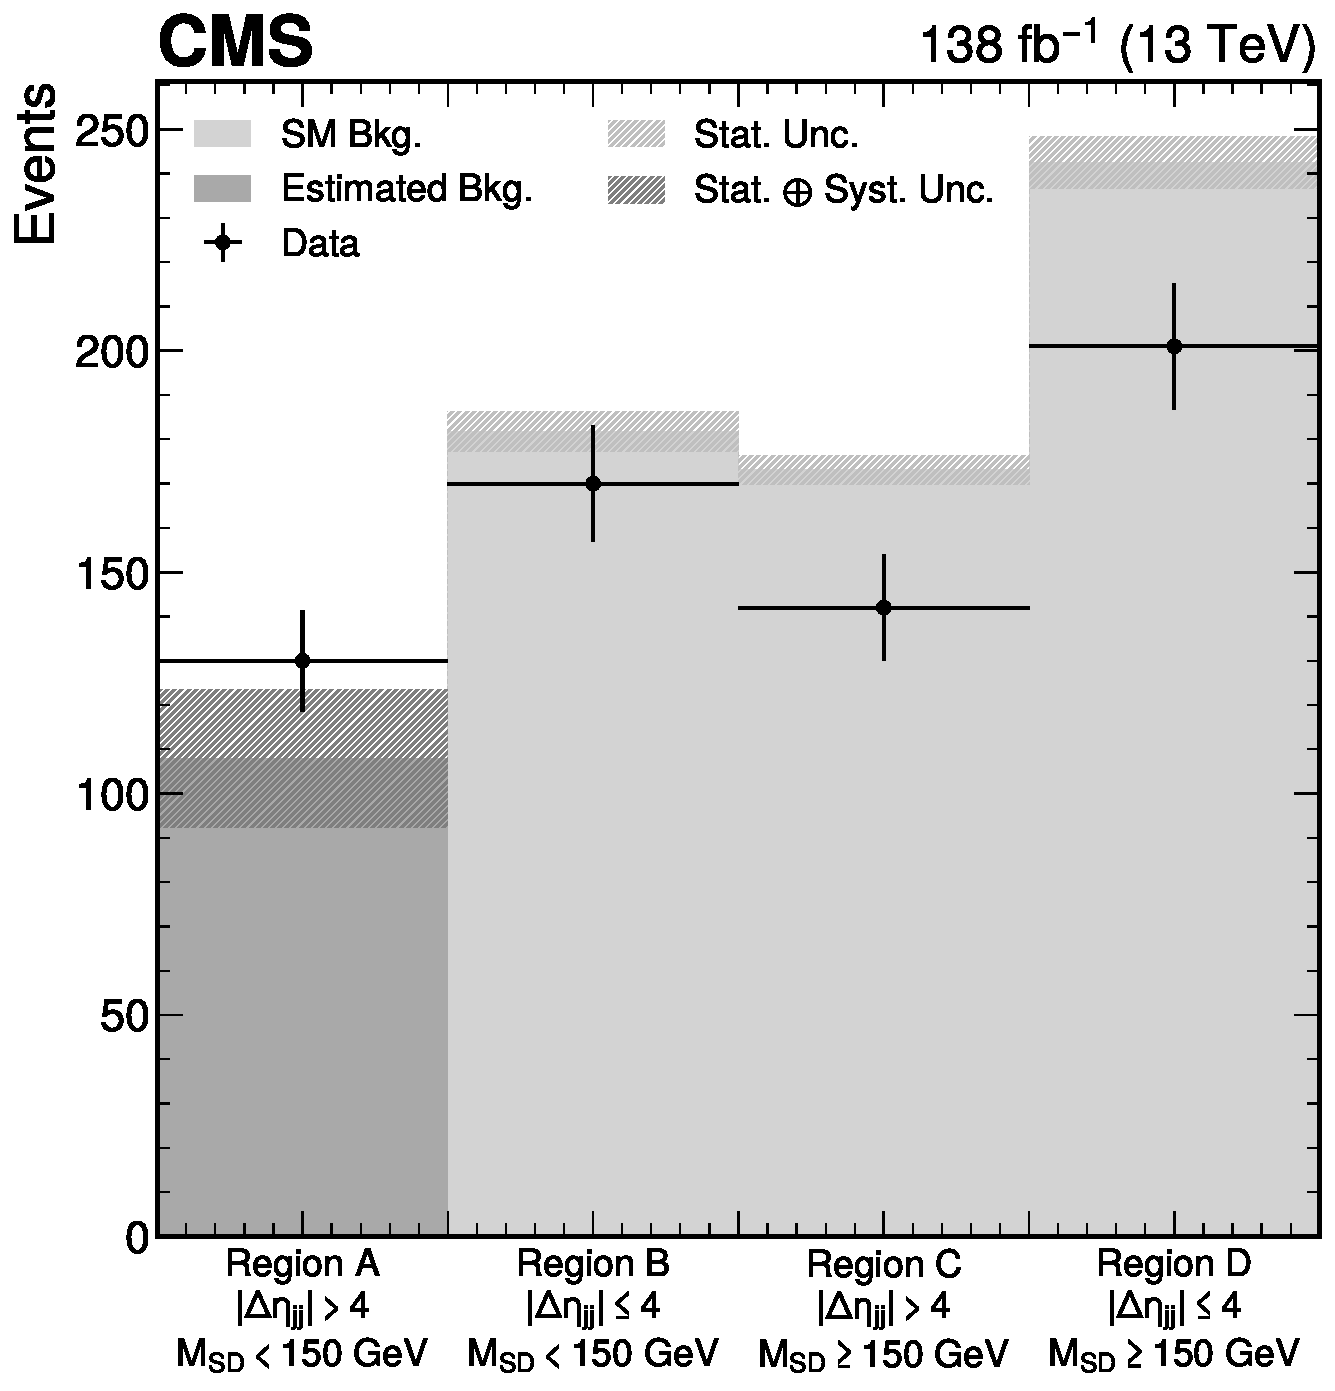
\includegraphics[width=0.45\textwidth]{fig/vbswh/regionsABCD_closure_unblinded.pdf}
    \caption[The data and MC yields plotted in regions A, B, C, and D.]{
        The data and MC yields plotted in regions A, B, C, and D as a 1-dimensional histogram. 
        In region A, the signal region, the background yield estimated from data is plotted instead of that predicted by MC. 
        Overall, there is good agreement between data and MC in regions B, C, and D, with the difference between data and MC never exceeding 2\std. 
    }
    \label{fig:vbswh_abcd_closure}
\end{figure}
However, the background composition is not consistent between the ABCD regions, and it is furthermore not known to high precision. 
The baseline systematic must be extended to cover the uncertainty in the background composition. 
In order to quantify this uncertainty, the yields for each of the next-to-leading backgrounds are varied within their respective statistical uncertainties, representing scenarios in which the contributions from each background are larger or smaller, and the closure of the method is recalculated. 
Based on how the closure varies for each scenario, a final systematic uncertainty of \BkgEstTotalSystErr\% is selected to cover the uncertainty in the background composition. 
Thus, the systematic and statistical uncertainties \Esyst and \Estat are
\begin{align*}
    \Esyst &\approx \BkgEstTotalSystErr\% \\
    \Estat &= \frac{\sqrt{\Bdata}}{\Bdata} \oplus \frac{\sqrt{\Cdata}}{\Cdata} \oplus \frac{\sqrt{\Ddata}}{\Ddata} \approx \BkgEstStatErr\%
\end{align*}
and the estimated background yield in the signal region is therefore given by 
\begin{equation*}
    \Adata^\text{pred} = \PredBkgNoCorrection \pm \PredBkgNoCorrectionStatErr \pm \PredBkgNoCorrectionSystErr
\end{equation*}
However, it can be seen in Fig.~\ref{fig:vbswh_abcd_corr} that the ABCD variables \detajj and \MSD are correlated.
This correlation is not evident in MC closure because it happens to ``cancel out,'' leading to the mild systematic over-prediction quantified above. 
To improve the reliability and accuracy of the method, a correction is computed in MC and applied to the transfer factor $\Cdata/\Ddata$ as follows:
\begin{equation*}
    \Adata^\text{pred} = \Bdata\times\frac{\Cdata}{\Ddata}\times\bigg(\frac{\AMC}{\CMC/\DMC}\bigg)
\end{equation*}
That is, the over-prediction of the ABCD method is measured in MC, i.e. the \BkgEstTotalSystErr\% computed before, but it is now used to adjust the transfer factor $\Cdata/\Ddata$ to account for the correlation between \MSD and \detajj. 
Moreover, in the $\MSD \geq 150\GeV$ sideband, comparison between data and MC shows that the correlation is well-modeled by MC (Fig.~\ref{fig:vbswh_abcd_corr_data_mc}), thus validating this correction. 
This trivially makes the method close exactly in MC, but by applying it to ABCD in data, the predicted background yield in the signal region is made more accurate, as the correlation was previously biasing the result.
Therefore, the final estimated background yield in the signal region is given by
\begin{equation*}
    \AdataPred = \PredBkg \pm \PredBkgStatErr \pm \PredBkgSystErr
\end{equation*}
where the systematic and statistical uncertainties are kept as \BkgEstTotalSystErr\% and \BkgEstStatErr\% respectively.

\begin{figure}[htb]
    \centering
    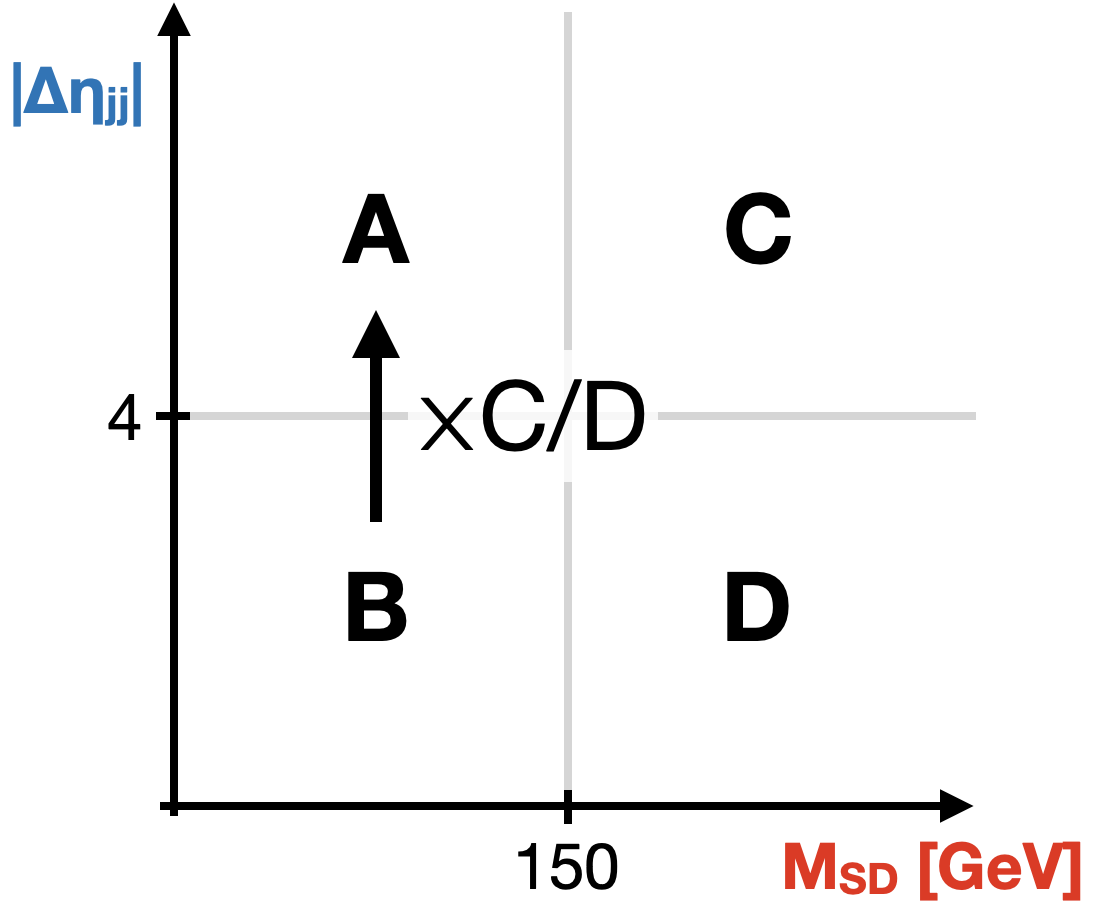
\includegraphics[width=0.45\textwidth]{fig/vbswh/abcd_cartoon.png}
    \caption{
        A sketch of regions A, B, C, and D used in the background estimation method.
    }
    \label{fig:vbswh_abcd_cartoon}
\end{figure}

\begin{figure}[htb]
    \centering
    \subfloat[]{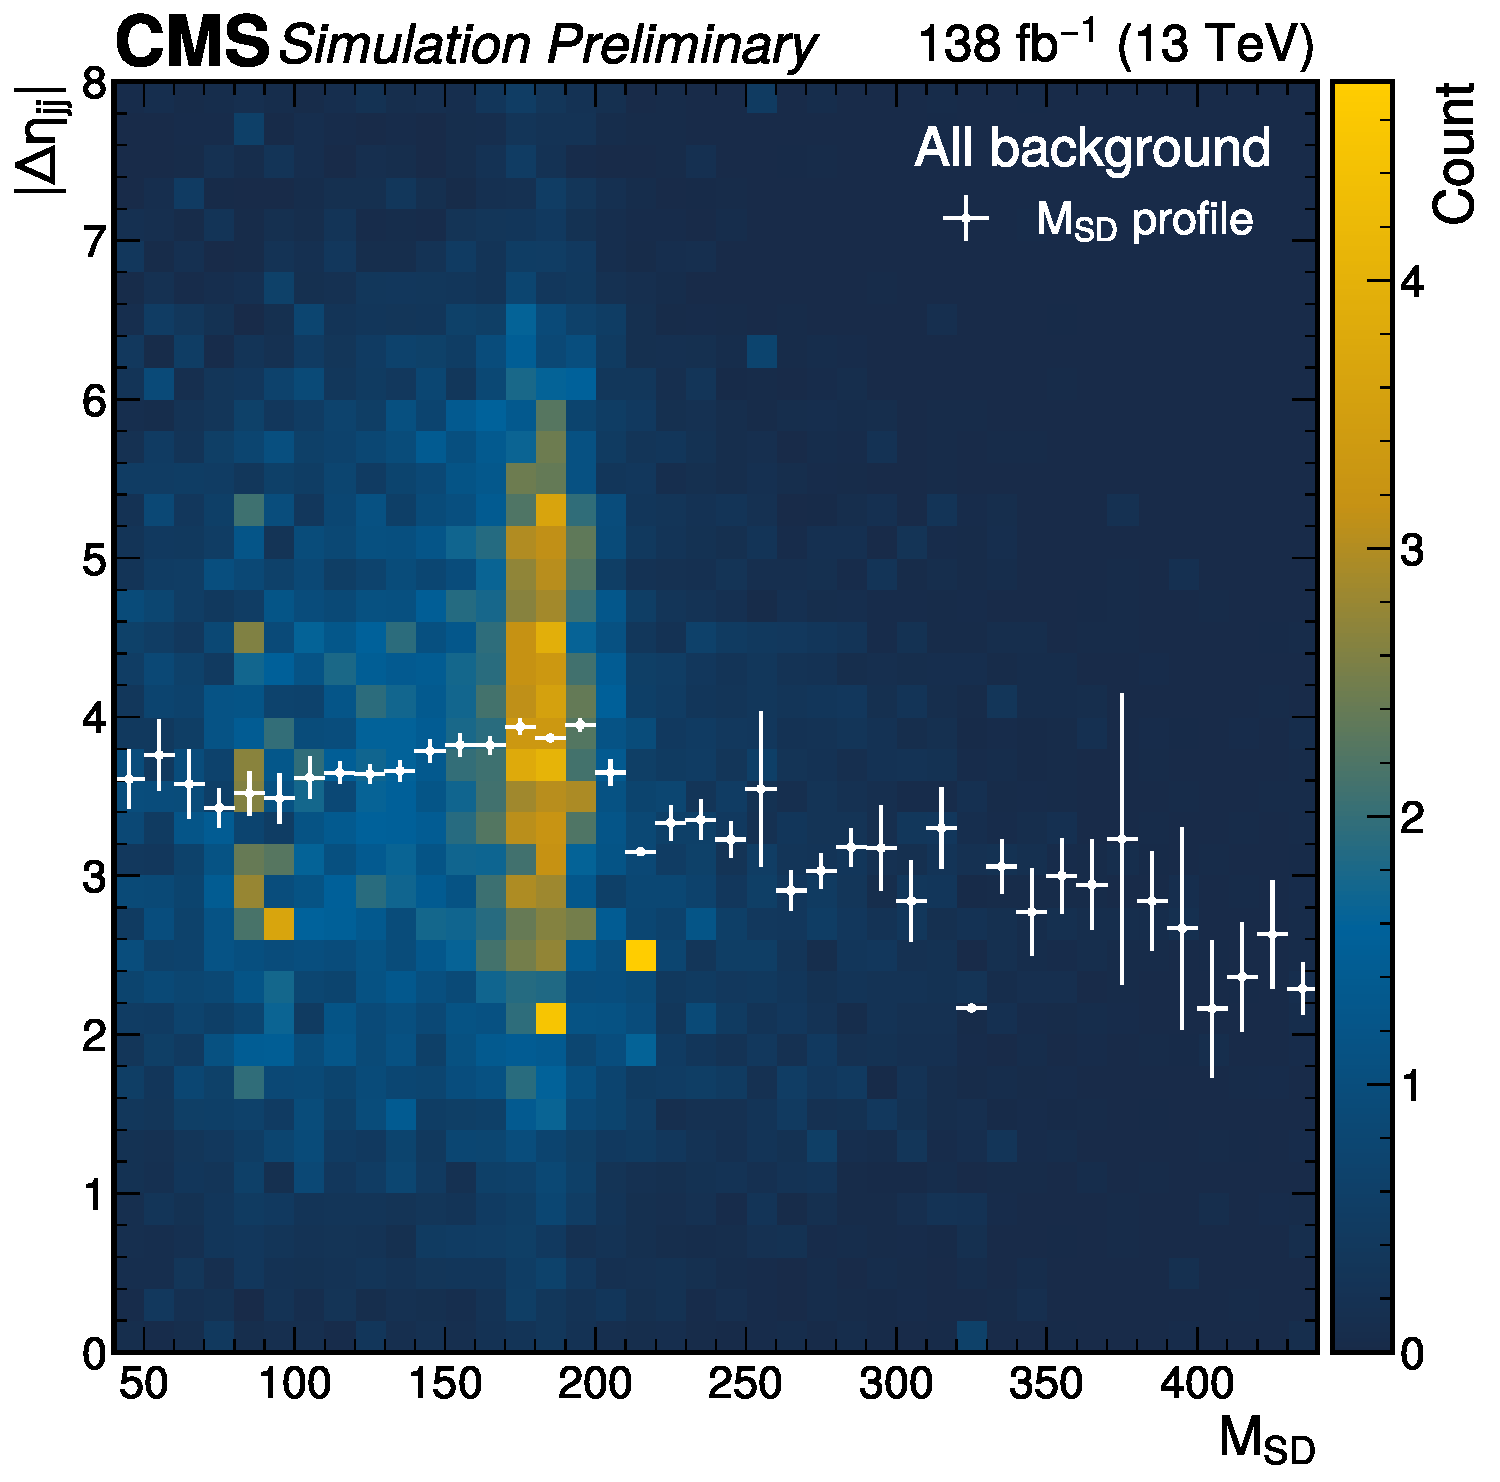
\includegraphics[width=0.45\textwidth]{fig/vbswh/correlation2D_1Dprofile_flipped.pdf}\label{fig:vbswh_abcd_corr}}
    \qquad
    \subfloat[]{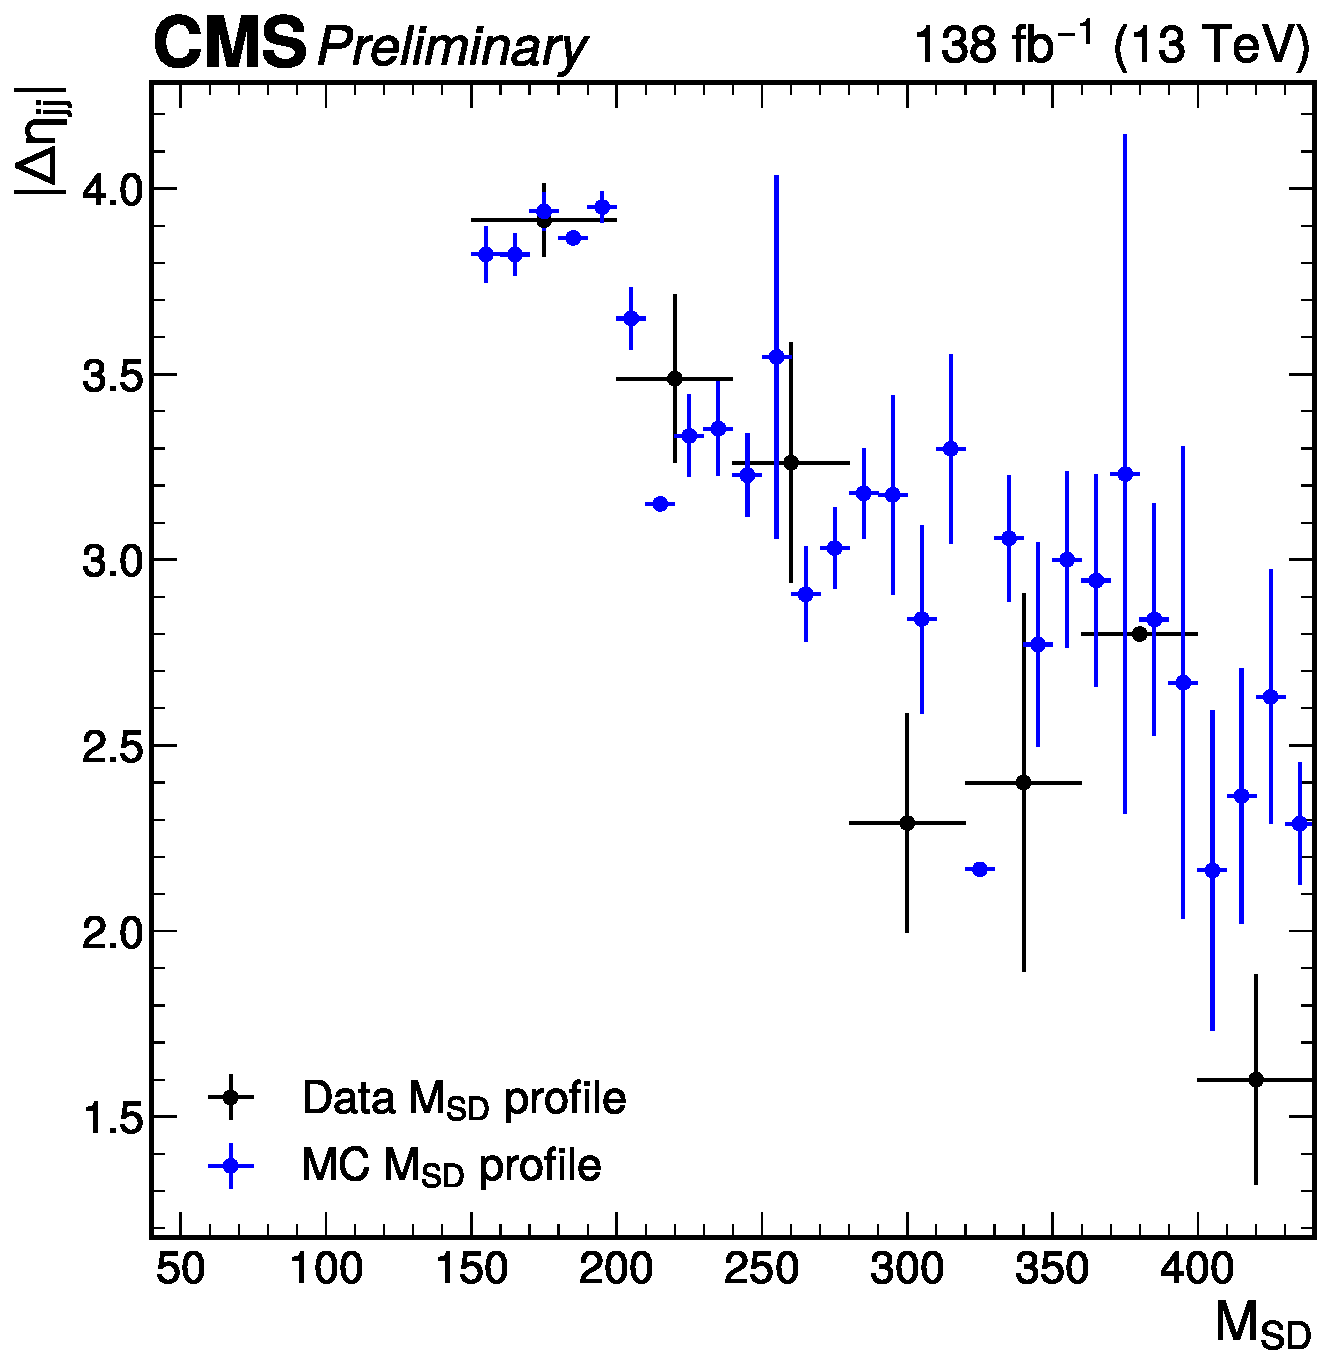
\includegraphics[width=0.45\textwidth]{fig/vbswh/correlation2D_1Dprofile_data_vs_mc.pdf}\label{fig:vbswh_abcd_corr_data_mc}}
    \caption[A 2-dimensional histogram of the ABCD variables \MSD and \detajj with a profile of \MSD]{
        A 2-dimensional histogram of the ABCD variables \MSD and \detajj with a profile of \MSD overlaid using only MC (left). 
        The downward trend in the profile plot indicates that there is a minor correlation between \MSD and \detajj. 
        The profile is compared between data and MC (right), and good agreement suggests that the correlation is at least well-modeled. 
        This correlation can thus be addressed with a correction derived from MC when applying the method in data, such that the background yield in the signal region is more accurately predicted.
    }
\end{figure}

\section{Results}
The background yield in the signal region estimated from data and the signal yield predicted by Monte Carlo simulation are tabulated in Table~\ref{tab:vbswh_yields}. 
Using these yields, and a thorough accounting of systematic uncertainties, we perform a maximum-likelihood fit~\cite{Cowan:2010js} using the \COMBINE statistical tool. 
Then, the exclusion significance and confidence level (CL) are extracted following the procedure described in Section~3.2 of Ref.~\cite{Aad2016MLM}.
In particular, we exclude the scenario where $\lambdaWZ = -1$ with an observed (expected) significance of 8.3\std (9.3\std), and we exclude all $\lambdaWZ < 0$ scenarios that were allowed by previous limits well beyond 5\std.
The results of this analysis therefore strongly indicate that \kW and \kZ have the same sign, representing another success of the Standard Model.

\begin{table}[htp]
    \centering
    \caption[VBS $\WH$ signal region yields]{
        Table of the signal region yields from signal MC, background estimated from data, and observed data along with their respective statistical and systematic uncertainties. 
        The systematic uncertainty for the signal quoted here is the sum in quadrature of all of the independent systematic uncertainties (percent errors) multiplied by the total yield.
        The observed yield is also tabulated. 
    }
    \label{tab:vbswh_yields}
    \begin{tabular}{c rclcl}
        \toprule
        Type       & Yield    & $\pm$ & stat.           & $\pm$ & syst.           \\ 
        \midrule
        Signal     & \ExpSig  & $\pm$ & \ExpSigStatErr  & $\pm$ & \ExpSigSystErr  \\
        Background & \PredBkg & $\pm$ & \PredBkgStatErr & $\pm$ & \PredBkgSystErr \\
        Observed   & \Obs     &       &                 &       &                 \\
        \bottomrule
    \end{tabular}
\end{table}

\begin{figure}[htb]
    \centering
    \subfloat[1D exclusion of $\lambdaWZ = -1$]{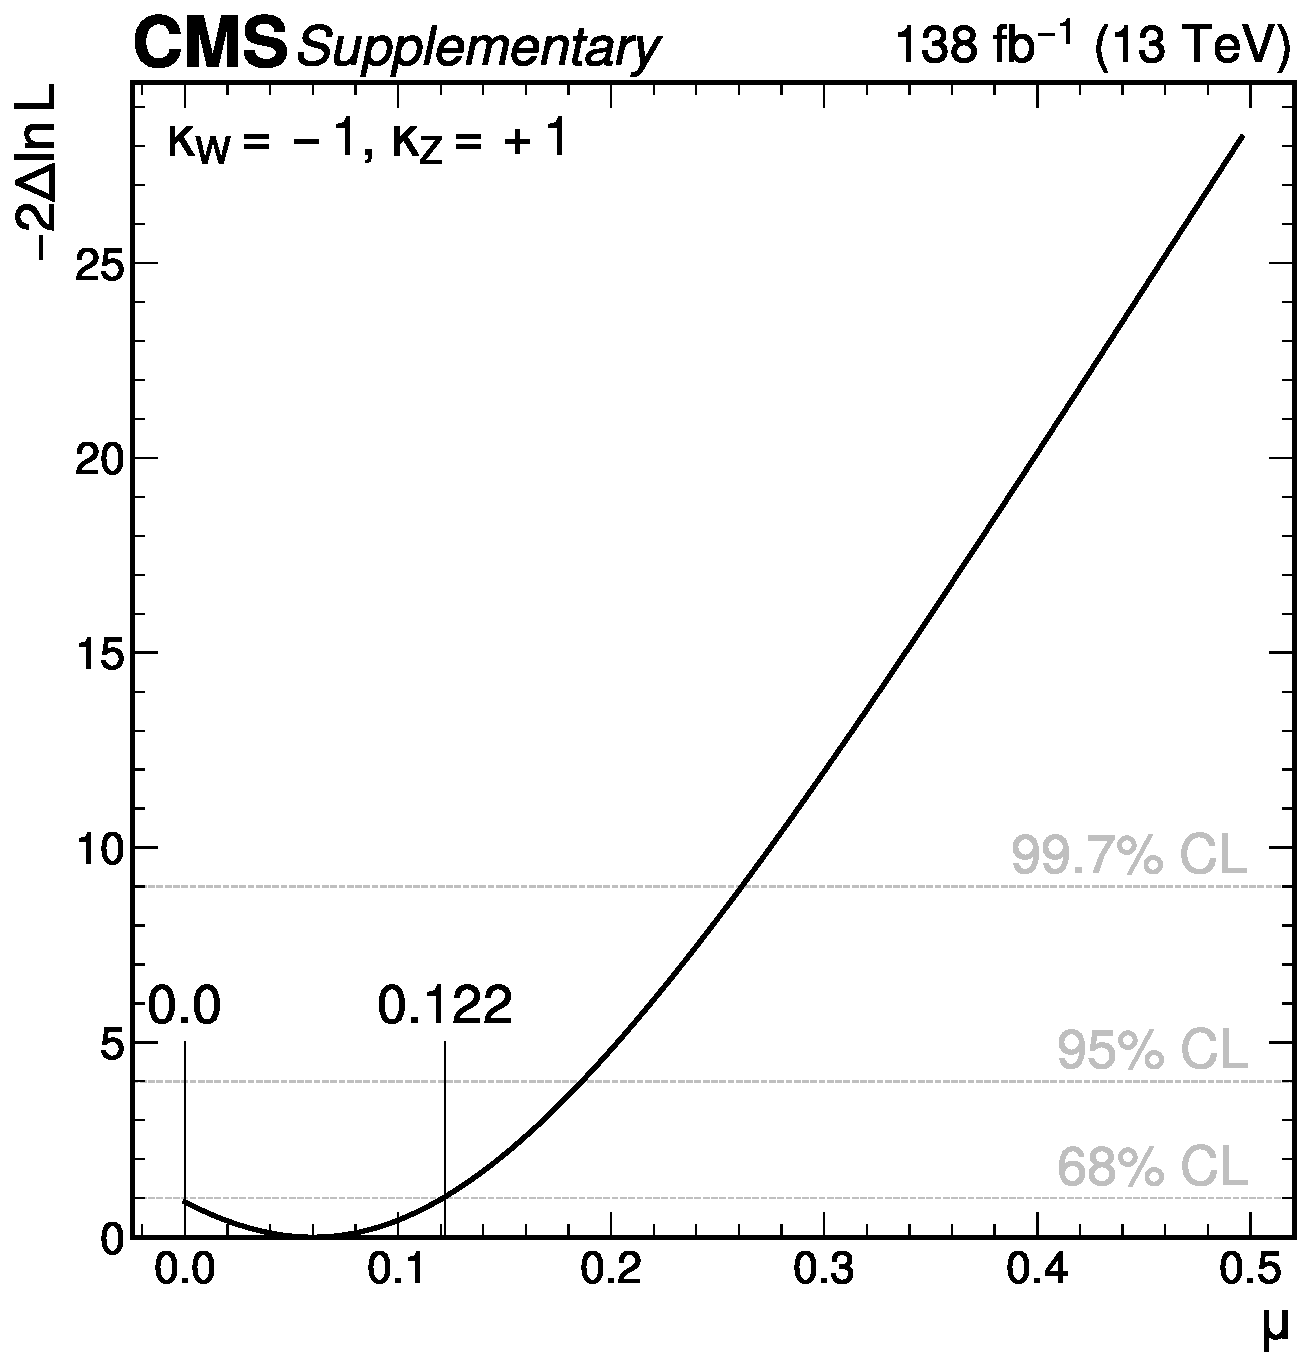
\includegraphics[width=0.445\textwidth,valign=c]{fig/vbswh/boosted_r_vs_m2deltaLogL_unblinded_zoom.pdf}\label{fig:vbswh_limit_1D}}
    \qquad
    \subfloat[2D exclusion of \lambdaWZ values]{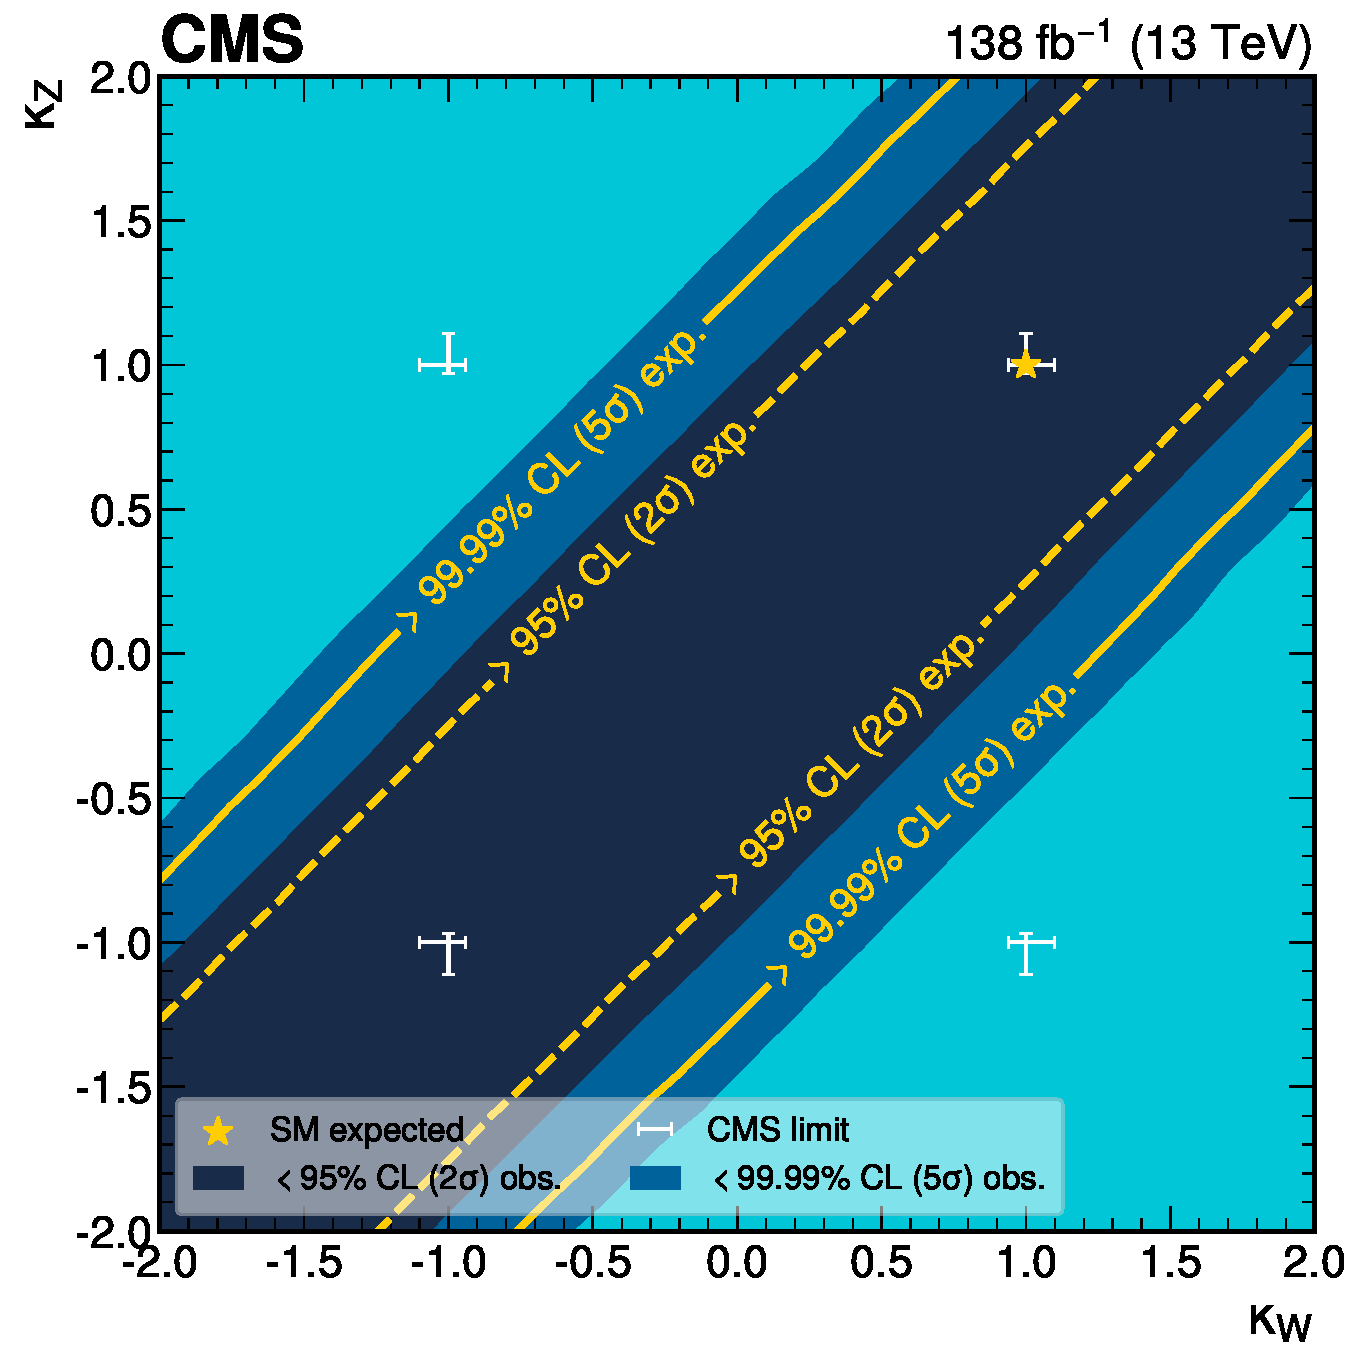
\includegraphics[width=0.455\textwidth,valign=c]{fig/vbswh/exclusion_2D_contours_unblinded.pdf}\label{fig:vbswh_limit_2D}}
    \caption[The 1D and 2D exclusion significance for BSM \lambdaWZ scenarios]{
        The negative-log-likelihood plotted as a function of the signal strength ($\mu$) for $\lambdaWZ = -1$, with the 68\% confidence interval labeled (a).
        The exclusion significance plotted as a function of \kW and \kZ with the previous best CMS limits plotted as white capped error bars (b).
        It is clear from these two plots (a) the $\lambdaWZ = -1$ scenario is excluded beyond 5\std and (b) opposite-sign scenarios ($\lambdaWZ < 0$) within previous CMS limits are also excluded beyond 5\std. 
    }
\end{figure}

\section{Acknowledgements}
This chapter is a partial reproduction of the paper ``Study of WH production through vector boson scattering and extraction of the relative sign of the W and Z couplings to the Higgs boson in proton-proton collisions at $\sqrt{s} = 13\TeV$,'' submitted to PLB (arXiv:2405.16566). 
The work was made possible by the technical and administrative staff that operate and maintain the CERN accelerator complex, the LHC, CMS itself, and the worldwide LHC computing grid that provides data storage and processing capabilities for every LHC analysis. 
